    \documentclass[12pt,a4paper]{article}
    \usepackage[utf8]{inputenc}
    \usepackage[T5]{fontenc}
    \usepackage[vietnamese]{babel}
    \usepackage{mathptmx}           % Times New Roman font
    \usepackage{geometry}
    \geometry{top=2cm, bottom=2cm, left=2.5cm, right=2cm, headheight=14.5pt}
    \usepackage{longtable}
    \usepackage{array}
    \usepackage{amssymb}
    \usepackage{indentfirst}
    \usepackage{booktabs}
    \usepackage{xcolor}
    \usepackage{colortbl}
    \usepackage{enumitem}
    \usepackage{graphicx}
    \usepackage{float}
    \usepackage{fancyhdr}
    \usepackage{lastpage}
    \usepackage{tikz}
    \usetikzlibrary{calc}
    
    % --- Cấu hình đường dẫn ảnh ---
    \graphicspath{{../images/}}
    
    \definecolor{headerblue}{RGB}{220,230,242}
    \definecolor{notegreen}{RGB}{234,250,234}
    
    % --- Cấu hình Header & Footer ---
    \pagestyle{fancy}
    \fancyhf{}
    \fancyhead[L]{\small \leftmark}
    \fancyhead[R]{\small Trang \thepage/\pageref{LastPage}}
    \renewcommand{\headrulewidth}{0.4pt}
    \renewcommand{\sectionmark}[1]{\markboth{#1}{}}
    \setcounter{tocdepth}{3}
    \setcounter{secnumdepth}{3}
    
\begin{document}

\begin{titlepage}
    \newgeometry{left=2cm, right=2cm, top=2cm, bottom=2cm}
    \begin{tikzpicture}[remember picture, overlay]
        \draw[line width = 2pt] ($(current page.north west) + (1.5cm,-1.5cm)$) rectangle ($(current page.south east) + (-1.5cm,1.5cm)$);
        \draw[line width = 0.5pt] ($(current page.north west) + (1.6cm,-1.6cm)$) rectangle ($(current page.south east) + (-1.6cm,1.6cm)$);
    \end{tikzpicture}

    \begin{center}
        \large \textbf{HỌC VIỆN CÔNG NGHỆ BƯU CHÍNH VIỄN THÔNG} \\
        \large \textbf{KHOA CÔNG NGHỆ THÔNG TIN 2} \\
        \large \textbf{BỘ MÔN THỰC TẬP CƠ SỞ} \\
        \vspace{0.5cm}
        \rule{3cm}{1pt} \\

        \vspace{1.2cm}
        \includegraphics[width=5.5cm]{Logo_PTIT_University.png} \\
        \vspace{1.5cm}

        \LARGE \textbf{BÁO CÁO CUỐI KỲ} \\
        \vspace{0.5cm}
        \Large \textbf{PHÂN TÍCH VÀ XÁC ĐỊNH YÊU CẦU HỆ THỐNG} \\
        \vspace{1cm}

        \begin{minipage}{14cm}
            \centering
            \large \textbf{Đề tài: Hệ thống nhận diện bệnh trên cây lúa dựa trên thuật toán học sâu CNN}
        \end{minipage}

        \vspace{2.5cm}

        \begin{tabular}{l l}
            \textbf{Giảng viên hướng dẫn:} & Cô Nguyễn Thị Bích Nguyên           \\
            \textbf{Nhóm:}                 & Nhóm 1                              \\
            \textbf{Lớp:}                  & E23CQCE01-N                         \\
            \textbf{Sinh viên thực hiện:}  & 1. Phan Tuấn Quốc Anh - N23DCCN003  \\
                                           & 2. Phạm Minh Khang - N23DCAT034     \\
                                           & 3. Nguyễn Lê Minh Phúc - N23DCDK058 \\
        \end{tabular}

        \vfill
        \large \textbf{TP. HỒ CHÍ MINH - 2026}
    \end{center}
    \restoregeometry
\end{titlepage}

\clearpage
\tableofcontents
\clearpage
\listoffigures
\clearpage
\listoftables
\clearpage

% ============================================================
\section{Tầm nhìn dự án}

\begin{longtable}{|l|p{11.5cm}|}
    \caption{Tầm nhìn dự án}                                                                                                                                 \\
    \hline
    \rowcolor{headerblue}
    \textbf{Mục}               & \textbf{Nội dung}                                                                                                           \\
    \hline
    \textbf{Nỗi đau hiện tại}  & Chẩn đoán bệnh trên cây lúa bằng mắt thường dẫn đến kết quả sai lệch, xử lý chậm trễ (1--3 ngày) và lạm dụng thuốc hóa học. \\
    \hline
    \textbf{Giải pháp đề xuất} & Ứng dụng trí tuệ nhân tạo (CNN) nhận diện bệnh qua hình ảnh, kết hợp dữ liệu thời tiết (GPS) và gợi ý dinh dưỡng thực vật.  \\
    \hline
    \textbf{Giá trị mang lại}  & Chẩn đoán nhanh (5--7 giây), chính xác, giảm phụ thuộc thuốc hóa học, nâng cao năng suất nông nghiệp.                       \\
    \hline
    \textbf{Ngoài phạm vi}     & Cảm biến IoT, thương mại điện tử, tích hợp ERP doanh nghiệp.                                                                \\
    \hline
\end{longtable}

% ============================================================
\section{Quy trình hiện tại và quy trình đề xuất}

\textbf{Quy trình hiện tại (As-Is):}
\begin{enumerate}
    \item Nông dân phát hiện triệu chứng bất thường trên lá lúa.
    \item Tự đoán bệnh dựa trên kinh nghiệm hoặc hỏi người xung quanh (mất 1--3 ngày).
    \item Mua thuốc bảo vệ thực vật theo cảm tính, dễ lạm dụng hóa chất.
\end{enumerate}

\textbf{Quy trình đề xuất (To-Be):}
\begin{enumerate}
    \item Nông dân chụp ảnh lá lúa bằng điện thoại.
    \item Hệ thống AI nhận diện bệnh trong 5--7 giây, khoanh vùng bệnh trên ảnh.
    \item Hệ thống gợi ý dinh dưỡng phù hợp với loại bệnh được phát hiện.
    \item Nông dân có thể phản hồi nếu kết quả chưa chính xác.
    \item Dữ liệu phản hồi được dùng để tái huấn luyện và nâng cấp mô hình AI.
\end{enumerate}

\hrulefill

% ============================================================
\section{Phạm vi áp dụng đề tài}
\begin{itemize}
    \item \textbf{Phạm vi nghiệp vụ:} Hệ thống số hóa quy trình chẩn đoán bệnh lúa qua hình ảnh bằng công nghệ nhận diện chuyên sâu. Hệ thống kết hợp phân tích hình ảnh và các thông số môi trường để đưa ra chẩn đoán chính xác. Kết hợp xây dựng kho tri thức về dinh dưỡng thực vật để gợi ý các loại vitamin và vi lượng cần bổ sung dựa trên việc truy xuất dữ liệu thông minh.
    \item \textbf{Phạm vi đối tượng:} Phục vụ Nông dân (nhận diện \& nhận gợi ý dinh dưỡng) và Quản trị viên (quản lý danh mục, cập nhật mô hình, quản lý kho kiến thức hệ thống).
    \item \textbf{Giới hạn đề tài:} Hệ thống tự chủ kho dữ liệu dinh dưỡng nội bộ. Đối với thông số môi trường, hệ thống sử dụng tọa độ vị trí (GPS) để tự động truy xuất dữ liệu thời tiết làm dữ liệu phụ trợ. Hỗ trợ nhận diện nhiều loại bệnh cùng lúc trên cùng một ảnh.
\end{itemize}

% ============================================================
\section{Các bước xác định yêu cầu}

Quá trình thực hiện xác định yêu cầu gồm 2 bước chính như sau:
\begin{itemize}
    \item \textbf{Bước 1:} Khảo sát hiện trạng, kết quả nhận được là các báo cáo về hiện trạng chẩn đoán bệnh trên cây lúa và nhu cầu bổ sung dinh dưỡng.
    \item \textbf{Bước 2:} Lập danh sách các yêu cầu, kết quả nhận được là danh sách các yêu cầu sẽ được thực hiện trên hệ thống máy tính.
\end{itemize}

\subsection{Đối tượng tham gia xác định yêu cầu}
Gồm 2 nhóm người:
\begin{itemize}
    \item \textbf{Chuyên viên tin học:} Thiết kế kiến trúc nhận diện thông minh, xây dựng kho kiến thức hệ thống và luồng xử lý truy xuất thông tin dinh dưỡng chính xác nhất.
    \item \textbf{Nhà chuyên môn (Kỹ sư nông nghiệp):} Cung cấp dữ liệu ảnh kèm thông số môi trường tương ứng, gán nhãn bệnh và trực tiếp biên soạn/chuẩn hóa bộ dữ liệu văn bản về vitamin/dinh dưỡng.
\end{itemize}
Hai nhóm người này phối hợp thật chặt chẽ để có thể xác định đầy đủ và chính xác các yêu cầu.

\hrulefill

\subsection{Khảo sát hiện trạng}

\subsubsection{Các hình thức thực hiện phổ biến}
\begin{itemize}
    \item \textbf{Quan sát:} Theo dõi và ghi hình quá trình cây lúa biểu hiện triệu chứng thiếu hụt dinh dưỡng hoặc mắc nhiều bệnh cùng lúc trên đồng ruộng dưới các điều kiện thời tiết khác nhau.
    \item \textbf{Khảo sát:} Khảo sát các người nông dân về mối liên hệ giữa các loại bệnh lúa, sự thiếu hụt dinh dưỡng và sự tác động của môi trường (nhiệt độ, độ ẩm).
    \item \textbf{Thu thập thông tin, tài liệu:} Thu thập tập dữ liệu ảnh lá lúa (kèm dữ liệu đặc tả về thời tiết/độ ẩm) và chuẩn bị bộ dữ liệu văn bản về dinh dưỡng thực vật.
\end{itemize}

\subsubsection{Quy trình thực hiện}
\textbf{A. Tìm hiểu tổng quan về thế giới thực:}
\begin{itemize}
    \item Quy mô hoạt động nông nghiệp, các bệnh dịch thường gặp.
    \item Xu hướng chuyển dịch sang bổ sung vitamin tăng sức đề kháng thay vì lạm dụng thuốc hóa học.
\end{itemize}

\textbf{B. Tìm hiểu hiện trạng tổ chức (cơ cấu tổ chức):}
\begin{itemize}
    \item Cơ cấu tổ chức bao gồm các chức danh: Quản trị viên (Quản lý dữ liệu bệnh, mô hình, tập dữ liệu dinh dưỡng), Nông dân (tải ảnh và mô tả tình trạng).
\end{itemize}

\textbf{C. Tìm hiểu hiện trạng nghiệp vụ:}
\begin{itemize}
    \item Việc tìm hiểu dựa trên: Thông tin đầu vào, Quá trình xử lý, Thông tin kết xuất.
    \item Xếp loại các nghiệp vụ vào 4 loại: Lưu trữ, Tính toán, Tra cứu, Kết xuất.
\end{itemize}

\hrulefill

% ============================================================
% DANH SÁCH BỆNH LÚA TRONG ĐỀ TÀI
% ============================================================
\subsection{Danh sách và mô tả các bệnh lúa trong đề tài}
Hệ thống được xây dựng để nhận diện 5 loại bệnh phổ biến trên cây lúa tại Việt Nam và khu vực Đông Nam Á. Thông tin về từng bệnh được tổng hợp từ tài liệu của Viện Lúa Quốc tế (IRRI) và các nghiên cứu chuyên ngành nông nghiệp.

\vspace{0.3cm}

\begin{longtable}{|
        >{\raggedright\arraybackslash}p{2.5cm}|
        >{\raggedright\arraybackslash}p{3cm}|
        >{\raggedright\arraybackslash}p{2cm}|
        >{\raggedright\arraybackslash}p{4cm}|
        >{\raggedright\arraybackslash}p{3cm}|}

    % --- 1. Tiêu đề và Đầu bảng (Trang đầu tiên) ---
    \caption{Danh sách và mô tả 5 bệnh lúa trong đề tài}
    \label{tab:diseases}                                                                                                                                                                                                                                                                                                                                               \\
    \hline
    \rowcolor{headerblue}
    \textbf{Tên bệnh}                                                                                                                                                                                                                      & \textbf{Tác nhân gây bệnh} & \textbf{Giai đoạn ảnh hưởng} & \textbf{Triệu chứng đặc trưng} & \textbf{Điều kiện phát sinh} \\ \hline
    \endfirsthead

    % --- 2. Đầu bảng (Cho các trang tiếp theo nếu bảng bị ngắt) ---
    \multicolumn{5}{c}%
    {{\tablename\ \thetable{} -- Tiếp theo trang trước}}                                                                                                                                                                                                                                                                                                               \\
    \hline
    \rowcolor{headerblue}
    \textbf{Tên bệnh}                                                                                                                                                                                                                      & \textbf{Tác nhân gây bệnh} & \textbf{Giai đoạn ảnh hưởng} & \textbf{Triệu chứng đặc trưng} & \textbf{Điều kiện phát sinh} \\ \hline
    \endhead

    % --- 3. Chân bảng (Cho các trang giữa nếu bảng bị ngắt) ---
    \hline \multicolumn{5}{|r|}{{Tiếp tục ở trang sau...}}                                                                                                                                                                                                                                                                                                             \\ \hline
    \endfoot

    % --- 4. Chân bảng (Trang cuối cùng của bảng) ---
    \hline
    \endlastfoot

    % ==========================================
    % NỘI DUNG BẢNG
    % ==========================================

    \textbf{Bạc lá} \newline \textit{Bacterial Blight}                                                                                                                                                                                     &
    Vi khuẩn \textit{Xanthomonas oryzae} pv.\ \textit{oryzae}                                                                                                                                                                              &
    Mạ đến trỗ bông                                                                                                                                                                                                                        &
    Lá non chuyển xanh xám và cuộn lại. Ở cây lớn, xuất hiện các vết sọc vàng cam dọc mép lá hoặc đầu lá, lan rộng dần thành màu vàng rơm và khô trắng. Mủ vi khuẩn màu vàng chảy ra khi cắt ngang phần bị bệnh.                           &
    Độ ẩm $>$ 70\%, nhiệt độ 25--34$^\circ$C, gió mạnh và mưa liên tục, bón thừa đạm.                                                                                                                                                                                                                                                                                  \\ \hline

    \textbf{Đốm nâu} \newline \textit{Brown Spot}                                                                                                                                                                                          &
    Nấm \textit{Bipolaris oryzae}                                                                                                                                                                                                          &
    Mạ đến chín sữa                                                                                                                                                                                                                        &
    Xuất hiện các đốm tròn hoặc bầu dục màu nâu trên lá, có tâm xám và viền đỏ nâu đặc trưng. Đốm có thể liên kết với nhau gây cháy toàn bộ lá. Hạt bị nhiễm có vết đen hoặc đổi màu (``pecky rice'').                                     &
    Độ ẩm 86--100\%, nhiệt độ 16--36$^\circ$C, lá ẩm liên tục 8--24 giờ, đất thiếu dinh dưỡng (đặc biệt là kali và silic).                                                                                                                                                                                                                                             \\ \hline

    \textbf{Đạo ôn} \newline \textit{Rice Blast}                                                                                                                                                                                           &
    Nấm \textit{Magnaporthe oryzae}                                                                                                                                                                                                        &
    Mạ đến trỗ bông                                                                                                                                                                                                                        &
    Vết bệnh hình thoi hoặc hình mắt én trên lá, tâm xám trắng, viền nâu đỏ, có quầng vàng xung quanh. Ở cổ bông (cổ cháy) gây lép hạt hàng loạt. Có thể giết chết cây ở giai đoạn mạ.                                                     &
    Độ ẩm $>$ 90\%, nhiệt độ ban ngày 25--28$^\circ$C và ban đêm 17--23$^\circ$C, sương mù buổi sáng, bón thừa đạm.                                                                                                                                                                                                                                                    \\ \hline

    \textbf{Vàng lùn lúa cỏ} \newline \textit{Rice Tungro}                                                                                                                                                                                 &
    2 loại virus: \textit{Rice tungro bacilliform virus} (RTBV) và \textit{Rice tungro spherical virus} (RTSV), lây truyền qua rầy xanh \textit{Nephotettix virescens}                                                                     &
    Đẻ nhánh đến làm đòng                                                                                                                                                                                                                  &
    Lá chuyển màu vàng hoặc vàng cam từ đầu lá lan vào. Cây còi cọc, thấp lùn, đẻ nhánh ít. Bông nhỏ, trỗ không thoát, hạt lép nhiều và có đốm nâu.                                                                                        &
    Nhiệt độ 25--35$^\circ$C, độ ẩm cao, mật độ rầy xanh lớn trên đồng. Rầy chỉ cần hút nhựa cây bệnh trong 5 phút là có thể truyền virus.                                                                                                                                                                                                                             \\ \hline

    \textbf{Khô vằn} \newline \textit{Sheath Blight}                                                                                                                                                                                       &
    Nấm \textit{Rhizoctonia solani}                                                                                                                                                                                                        &
    Đẻ nhánh đến chín sữa                                                                                                                                                                                                                  &
    Vết bệnh hình bầu dục hoặc không đều trên bẹ lá, ban đầu màu xanh xám ngấm nước, sau chuyển xám trắng với viền nâu. Bệnh lan từ bẹ lên phiến lá và sang các nhánh lân cận. Có thể tìm thấy hạch nấm (sclerotia) màu nâu trên vết bệnh. &
    Độ ẩm 85--100\%, nhiệt độ 28--32$^\circ$C, mùa mưa, mật độ sạ dày, ruộng ngập nước.                                                                                                                                                                                                                                                                                \\
\end{longtable}

\subsubsection{Hình ảnh minh họa thực tế các loại bệnh hại trong đề tài}
Để phục vụ công tác xây dựng tập dữ liệu huấn luyện và hỗ trợ giao diện chẩn đoán trực quan cho người dùng, dưới đây là hình ảnh thực tế biểu hiện lâm sàng của 5 loại bệnh lúa trong đề tài được thu thập từ đồng ruộng:

\begin{figure}[H]
    \centering
    \begin{minipage}{0.48\textwidth}
        \centering
        \includegraphics[width=\textwidth,height=5.8cm,keepaspectratio]{bacterial-leaf-blight.jpg}
        \caption{Triệu chứng bệnh Bạc lá (Bacterial Blight)}
        \label{fig:bacterial-leaf-blight}
    \end{minipage}
    \hfill
    \begin{minipage}{0.48\textwidth}
        \centering
        \includegraphics[width=\textwidth,height=5.8cm,keepaspectratio]{brown-spot.jpg}
        \caption{Triệu chứng bệnh Đốm nâu (Brown Spot)}
        \label{fig:brown-spot}
    \end{minipage}
\end{figure}

\begin{figure}[H]
    \centering
    \begin{minipage}{0.48\textwidth}
        \centering
        \includegraphics[width=\textwidth,height=5.8cm,keepaspectratio]{blast-leaf.jpg}
        \caption{Triệu chứng bệnh Đạo ôn (Rice Blast)}
        \label{fig:blast-leaf}
    \end{minipage}
    \hfill
    \begin{minipage}{0.48\textwidth}
        \centering
        \includegraphics[width=\textwidth,height=5.8cm,keepaspectratio]{tungro.jpg}
        \caption{Triệu chứng bệnh Vàng lùn lúa cỏ (Rice Tungro)}
        \label{fig:tungro}
    \end{minipage}
\end{figure}

\begin{figure}[H]
    \centering
    \includegraphics[width=0.5\textwidth,height=5.8cm,keepaspectratio]{sheath-blight.jpg}
    \caption{Triệu chứng bệnh Khô vằn (Sheath Blight)}
    \label{fig:sheath-blight}
\end{figure}



\subsection{Lập danh sách các yêu cầu}
\subsubsection{Xác định yêu cầu chức năng nghiệp vụ}

Dựa trên kết quả khảo sát hiện trạng, hệ thống xác định 2 nhóm người dùng chính với các yêu cầu chức năng nghiệp vụ tương ứng:

\begin{longtable}{|c|p{2.5cm}|p{2cm}|p{8cm}|}
    \hline
    \rowcolor{headerblue}
    \textbf{STT} & \textbf{Tên tác nhân} & \textbf{Mã số} & \textbf{Mô tả vai trò \& mục đích sử dụng}                                                                                      \\
    \hline
    \endhead
    1            & Nông dân              & ND             &
    Người dùng cuối, sử dụng ứng dụng trên thiết bị di động để chẩn đoán bệnh lúa qua hình ảnh, xem gợi ý dinh dưỡng, tra cứu lịch sử chẩn đoán, gửi phản hồi kết quả và tham gia diễn đàn. \\
    \hline
    2            & Quản trị viên         & AD             &
    Người vận hành và duy trì hệ thống. Quản lý danh mục bệnh lúa, kho tri thức dinh dưỡng, tài khoản người dùng, xử lý phản hồi và cập nhật mô hình AI.                                    \\
    \hline
\end{longtable}

Chi tiết yêu cầu chức năng nghiệp vụ của từng nhóm người dùng được trình bày trong các mục tiếp theo.

\subsubsection{Xác định yêu cầu chức năng hệ thống và yêu cầu chất lượng}

\textbf{Bảng yêu cầu chức năng hệ thống:}
\begin{longtable}{|c|l|p{9.5cm}|l|}
    \hline
    \rowcolor{headerblue}
    \textbf{STT} & \textbf{Nội dung}  & \textbf{Mô tả chi tiết}                                                                            & \textbf{Ghi chú} \\
    \hline
    \endhead
    1            & Tích hợp thời tiết & Truy xuất dữ liệu thời tiết dựa trên tọa độ thực tế của nông dân để cung cấp bối cảnh môi trường.  &                  \\
    \hline
    2            & Quản lý tri thức   & Hệ thống đồng bộ các hướng dẫn dinh dưỡng để AI có thể tư vấn linh hoạt.                           &                  \\
    \hline
    3            & Bảo mật dữ liệu    & Mật khẩu được bảo mật an toàn. Toàn bộ ảnh và dữ liệu thực tế được lưu trữ phục vụ tái huấn luyện. &                  \\
    \hline
    4            & Gửi mã xác thực    & Tự động gửi mã xác thực qua email cho các luồng xác minh tài khoản.                                &                  \\
    \hline
\end{longtable}

\textbf{Bảng yêu cầu về chất lượng hệ thống:}
\begin{longtable}{|c|l|l|p{6.5cm}|l|}
    \hline
    \rowcolor{headerblue}
    \textbf{STT} & \textbf{Nội dung} & \textbf{Tiêu chuẩn} & \textbf{Mô tả chi tiết}                                                    & \textbf{Ghi chú} \\
    \hline
    \endhead
    1            & Cập nhật mô hình  & Tiến hóa            & Có thể thay thế mô hình nhận diện mới mà không làm gián đoạn người dùng.   &                  \\
    \hline
    2            & Tính tiện dụng    & Tiện dụng           & Giao diện tối ưu cho thiết bị di động, thông báo rõ ràng bằng tiếng Việt.  &                  \\
    \hline
    3            & Tốc độ xử lý      & Hiệu quả            & Phản hồi kết quả chẩn đoán trong vòng 5--7 giây.                           &                  \\
    \hline
    4            & Độ tương thích    & Tương thích         & Hoạt động ổn định trên các trình duyệt phổ biến của điện thoại thông minh. &                  \\
    \hline
    5            & Tính kịp thời     & Hiệu quả            & Mã xác thực gửi đến người dùng trong vòng 30 giây.                         &                  \\
    \hline
\end{longtable}

\hrulefill

% ============================================================
% NGƯỜI DÙNG: NÔNG DÂN
% ============================================================
\section{Người dùng --- Nông dân (Mã số: ND)}

\textbf{Định nghĩa:} Người sử dụng hệ thống với mục đích chẩn đoán bệnh trên cây lúa qua hình ảnh, xem gợi ý dinh dưỡng và phản hồi kết quả chẩn đoán.

\vspace{0.3cm}
\textbf{1. Bảng yêu cầu chức năng nghiệp vụ}

\begin{longtable}{|
        c|
        >{\raggedright\arraybackslash}p{3.2cm}|
        >{\raggedright\arraybackslash}p{2.2cm}|
        >{\raggedright\arraybackslash}p{2.4cm}|
        >{\raggedright\arraybackslash}p{2.6cm}|
        >{\raggedright\arraybackslash}p{2.6cm}|}

    \caption{Bảng yêu cầu chức năng nghiệp vụ --- Nông dân} \label{tab:nd-ycnv}                                                                                       \\
    \hline
    \rowcolor{headerblue}
    \textbf{STT} & \textbf{Công việc}             & \textbf{Loại công việc} & \textbf{Quy định/CT liên quan} & \textbf{Biểu mẫu liên quan} & \textbf{Ghi chú}         \\
    \hline
    \endfirsthead

    \multicolumn{6}{c}%
    {{\tablename\ \thetable{} -- Tiếp theo trang trước}}                                                                                                              \\
    \hline
    \rowcolor{headerblue}
    \textbf{STT} & \textbf{Công việc}             & \textbf{Loại công việc} & \textbf{Quy định/CT liên quan} & \textbf{Biểu mẫu liên quan} & \textbf{Ghi chú}         \\
    \hline
    \endhead

    \hline \multicolumn{6}{|r|}{{Tiếp tục ở trang sau...}}                                                                                                            \\ \hline
    \endfoot

    \hline
    \endlastfoot

    \multicolumn{6}{|l|}{\cellcolor{notegreen}\textbf{I. Quản lý tài khoản}}                                                                                          \\
    \hline
    1            & Đăng ký tài khoản              & Lưu trữ                 & QĐ-ND-01.1                     & ND\_BM 1                    &                          \\
    \hline
    2            & Đăng nhập hệ thống             & Tra cứu                 & QĐ-ND-01.2                     & ND\_BM 1b                   &                          \\
    \hline
    3            & Thiết lập tài khoản lần đầu    & Lưu trữ                 & QĐ-ND-01.3                     &                             & Chỉ thực hiện 1 lần      \\
    \hline
    4            & Khôi phục mật khẩu             & Lưu trữ                 & QĐ-ND-01.4                     &                             &                          \\
    \hline
    5            & Đổi mật khẩu                   & Lưu trữ                 & QĐ-ND-01.5                     & ND\_BM 1c                   &                          \\
    \hline
    6            & Đăng xuất hệ thống             & Lưu trữ                 & QĐ-ND-01.6                     &                             &                          \\
    \hline
    \multicolumn{6}{|l|}{\cellcolor{notegreen}\textbf{II. Hồ sơ cá nhân}}                                                                                             \\
    \hline
    7            & Xem thông tin cá nhân          & Tra cứu                 & QĐ-ND-02.1                     &                             &                          \\
    \hline
    8            & Chỉnh sửa thông tin cá nhân    & Lưu trữ                 & QĐ-ND-02.2                     & ND\_BM 2                    &                          \\
    \hline
    \multicolumn{6}{|l|}{\cellcolor{notegreen}\textbf{III. Quản lý ruộng đất (Field Book)}}                                                                           \\
    \hline
    9            & Xem danh sách ruộng            & Tra cứu                 & QĐ-ND-03.1                     &                             &                          \\
    \hline
    10           & Thêm ruộng đất mới             & Lưu trữ                 & QĐ-ND-03.2                     &                             &                          \\
    \hline
    11           & Chỉnh sửa ruộng đất            & Lưu trữ                 & QĐ-ND-03.3                     &                             &                          \\
    \hline
    12           & Xóa ruộng đất                  & Lưu trữ                 & QĐ-ND-03.4                     &                             &                          \\
    \hline
    13           & Thiết lập ruộng mặc định       & Lưu trữ                 & QĐ-ND-03.5                     &                             &                          \\
    \hline
    \multicolumn{6}{|l|}{\cellcolor{notegreen}\textbf{IV. Chẩn đoán bệnh lúa}}                                                                                        \\
    \hline
    14           & Gửi ảnh chẩn đoán              & Lưu trữ                 & QĐ-ND-04.1                     & ND\_BM 3                    &                          \\
    \hline
    15           & Chọn vị trí ruộng              & Lưu trữ                 & QĐ-ND-04.2                     &                             & Tùy chọn, không bắt buộc \\
    \hline
    16           & Mô tả triệu chứng              & Lưu trữ                 & QĐ-ND-04.3                     &                             & Tùy chọn, không bắt buộc \\
    \hline
    17           & Nhập thông số thực địa         & Lưu trữ                 & QĐ-ND-04.4                     & ND\_BM 3b                   & Tùy chọn, không bắt buộc \\
    \hline
    18           & Xem kết quả chẩn đoán          & Tra cứu, Tính toán      & QĐ-ND-04.5                     &                             &                          \\
    \hline
    \multicolumn{6}{|l|}{\cellcolor{notegreen}\textbf{V. Tra cứu lịch sử}}                                                                                            \\
    \hline
    19           & Tra cứu lịch sử chẩn đoán      & Tra cứu                 & QĐ-ND-05.1                     &                             &                          \\
    \hline
    20           & Xem chi tiết một lần chẩn đoán & Tra cứu                 & QĐ-ND-05.2                     &                             &                          \\
    \hline
    \multicolumn{6}{|l|}{\cellcolor{notegreen}\textbf{VI. Phản hồi kết quả}}                                                                                          \\
    \hline
    21           & Gửi phản hồi kết quả           & Lưu trữ                 & QĐ-ND-06.1                     & ND\_BM 4                    &                          \\
    \hline
    22           & Xem kết quả xử lý phản hồi     & Tra cứu                 & QĐ-ND-06.2                     &                             &                          \\
    \hline
    \multicolumn{6}{|l|}{\cellcolor{notegreen}\textbf{VII. Diễn đàn}}                                                                                                 \\
    \hline
    23           & Xem danh sách bài viết         & Tra cứu                 & QĐ-ND-07.1                     &                             & Không cần đăng nhập      \\
    \hline
    24           & Đăng bài viết mới              & Lưu trữ                 & QĐ-ND-07.2                     &                             &                          \\
    \hline
    25           & Chỉnh sửa bài viết             & Lưu trữ                 & QĐ-ND-07.3                     &                             &                          \\
    \hline
    26           & Xóa bài viết                   & Lưu trữ                 & QĐ-ND-07.4                     &                             &                          \\
    \hline
    27           & Xem chi tiết bài viết          & Tra cứu                 & QĐ-ND-07.5                     &                             & Không cần đăng nhập      \\
    \hline
    28           & Bình luận \& Phản hồi          & Lưu trữ                 & QĐ-ND-07.6                     &                             &                          \\
    \hline
    29           & Chỉnh sửa / Xóa bình luận      & Lưu trữ                 & QĐ-ND-07.7                     &                             &                          \\
    \hline
    30           & Vote bài viết \& bình luận     & Lưu trữ                 & QĐ-ND-07.8                     &                             &                          \\
    \hline
\end{longtable}

% ============================================================
\vspace{0.3cm}
\textbf{2. Bảng Quy định / Công thức liên quan --- Nông dân}

% ---- QĐ-ND-01 ----
\vspace{0.3cm}
\noindent\textbf{QĐ-ND-01 --- Quy định Tài khoản}

\begin{longtable}{|
        >{\raggedright\arraybackslash}p{2.2cm}|
        >{\raggedright\arraybackslash}p{2.8cm}|
        >{\raggedright\arraybackslash}p{9.8cm}|}
    \hline
    \rowcolor{headerblue}
    \textbf{Mã quy định} & \textbf{Chức năng}                   & \textbf{Quy trình \& Ràng buộc}                                                                                                                                                                                                                        \\
    \hline
    \endfirsthead
    \multicolumn{3}{c}{{\tablename\ -- Tiếp theo trang trước}}                                                                                                                                                                                                                                                           \\
    \hline
    \rowcolor{headerblue}
    \textbf{Mã quy định} & \textbf{Chức năng}                   & \textbf{Quy trình \& Ràng buộc}                                                                                                                                                                                                                        \\
    \hline
    \endhead
    \hline \multicolumn{3}{|r|}{{Tiếp tục ở trang sau...}}                                                                                                                                                                                                                                                               \\ \hline
    \endfoot
    \hline
    \endlastfoot
    \textbf{QĐ-ND-01.1}  & \textbf{Đăng ký tài khoản}           &
    Nông dân phải cung cấp đầy đủ và hợp lệ các thông tin sau:
    \begin{itemize}[leftmargin=*,topsep=2pt,itemsep=1pt]
        \item \textbf{Tên đăng nhập:} phải là duy nhất trong hệ thống, không chứa khoảng trắng, chỉ gồm chữ cái, chữ số và dấu gạch dưới.
        \item \textbf{Email:} đúng định dạng email, chưa tồn tại trong hệ thống.
        \item \textbf{Mật khẩu:} Mật khẩu phải đáp ứng đủ các ràng buộc sau: tối thiểu 8 ký tự; ít nhất 1 chữ viết hoa (A--Z); ít nhất 1 chữ viết thường (a--z); ít nhất 1 ký tự đặc biệt (ví dụ: @, \$, !, \%, *, ?, \&).
        \item \textbf{Xác nhận mật khẩu:} phải gõ lại chính xác giống mật khẩu đã nhập.
        \item \textbf{Đồng ý điều khoản:} phải tích chọn checkbox xác nhận ``Tôi đồng ý với các điều khoản dịch vụ và chính sách bảo mật''. Đây là trường bắt buộc để kích hoạt nút Đăng ký.
    \end{itemize}
    \textbf{Quy tắc xử lý:} Nút ``Đăng ký'' chỉ hiển thị trạng thái hoạt động (active) khi nông dân đã điền đầy đủ thông tin hợp lệ và tích chọn checkbox. Hệ thống gửi liên kết xác thực hoặc mã OTP về email để kích hoạt tài khoản. Sau khi đăng ký thành công, hệ thống tự động chuyển nông dân tới trang đăng nhập. \\
    \hline
    \textbf{QĐ-ND-01.2}  & \textbf{Đăng nhập}                   &
    Hệ thống hỗ trợ 2 hình thức đăng nhập:
    \begin{itemize}[leftmargin=*,topsep=2pt,itemsep=1pt]
        \item \textbf{Đăng nhập thông thường (bằng tài khoản đã đăng ký):} nhập tên đăng nhập hoặc email và mật khẩu tương ứng. Nếu đăng nhập sai, hệ thống chỉ hiển thị thông báo chung ``Tên đăng nhập hoặc mật khẩu không chính xác'' mà không chỉ rõ trường nào sai.
        \item \textbf{Đăng nhập bằng Google:} nông dân chọn tùy chọn ``Đăng nhập với Google'' và xác thực qua tài khoản Google. Hệ thống tự động tạo tài khoản nếu email Google chưa tồn tại trong hệ thống.
    \end{itemize}
    \textbf{Quy tắc xử lý:} Hệ thống cấp chứng chỉ phiên làm việc (JWT) sau khi xác thực thành công. Nếu là lần đầu đăng nhập, hệ thống chuyển nông dân sang luồng Thiết lập tài khoản lần đầu (QĐ-ND-01.3). Các lần đăng nhập tiếp theo, hệ thống chuyển thẳng tới trang chẩn đoán bệnh.                                \\
    \hline
    \textbf{QĐ-ND-01.3}  & \textbf{Thiết lập tài khoản lần đầu} &
    Luồng ``Lúa Khỏe Onboarding'' chỉ được kích hoạt duy nhất một lần sau khi nông dân đăng nhập thành công lần đầu tiên. Hệ thống phân nhánh theo hình thức đăng nhập:

    \textbf{Nhánh 1 --- Tài khoản Google (2 bước):}
    \begin{enumerate}[leftmargin=*,topsep=2pt,itemsep=1pt]
        \item \textbf{Bước 1 --- Thiết lập mật khẩu:} Nông dân nhập mật khẩu mới và xác nhận mật khẩu. Mật khẩu phải đáp ứng đủ các ràng buộc sau: tối thiểu 8 ký tự; ít nhất 1 chữ viết hoa (A--Z); ít nhất 1 chữ viết thường (a--z); ít nhất 1 ký tự đặc biệt (ví dụ: @, \$, !, \%, *, ?, \&).
        \item \textbf{Bước 2 --- Thiết lập vị trí ruộng mặc định:} Hệ thống hiển thị bản đồ với 2 tùy chọn: (a) \textbf{Lấy vị trí hiện tại} --- tự động định vị GPS của thiết bị và ghim lên bản đồ; (b) \textbf{Chọn vị trí trên bản đồ} --- nông dân kéo thả ghim để chọn vị trí ruộng thủ công. Bước này không bắt buộc, nông dân có thể bỏ qua.
    \end{enumerate}

    \textbf{Nhánh 2 --- Tài khoản thông thường (1 bước):}
    \begin{enumerate}[leftmargin=*,topsep=2pt,itemsep=1pt]
        \item \textbf{Bước 2 --- Thiết lập vị trí ruộng mặc định:} Thực hiện tương tự Bước 2 của Nhánh 1. Bước thiết lập mật khẩu được bỏ qua vì mật khẩu đã được tạo khi đăng ký.
    \end{enumerate}

    \textbf{Quy tắc xử lý:} Sau khi hoàn tất Onboarding, hệ thống lưu tọa độ GPS mặc định vào hồ sơ người dùng (nếu có) và chuyển nông dân tới trang chẩn đoán bệnh. Thông tin vị trí này được tự động sử dụng cho các lần chẩn đoán tiếp theo (QĐ-ND-04.2).                                                             \\
    \hline
    \textbf{QĐ-ND-01.4}  & \textbf{Khôi phục mật khẩu}          &
    Thực hiện theo 4 bước tuần tự:
    \begin{enumerate}[leftmargin=*,topsep=2pt,itemsep=1pt]
        \item Nhập \textbf{địa chỉ email} đã đăng ký trong hệ thống.
        \item Hệ thống gửi \textbf{mã OTP} 6 chữ số về email --- hiệu lực 10 phút. Nhập sai 3 lần thì hủy mã.
        \item Nhập \textbf{mật khẩu mới} --- không được trùng mật khẩu cũ, đáp ứng độ mạnh như khi đăng ký.
        \item Nhập \textbf{xác nhận mật khẩu mới} --- phải gõ chính xác giống bước 3.
    \end{enumerate}
    \textbf{Quy tắc xử lý:} Sau khi đặt lại mật khẩu thành công, hệ thống tự động hủy tất cả phiên đăng nhập cũ trên các thiết bị khác và chuyển nông dân về trang đăng nhập.                                                                                                                                            \\
    \hline
    \textbf{QĐ-ND-01.5}  & \textbf{Đổi mật khẩu}                &
    Thực hiện theo các bước sau:
    \begin{enumerate}[leftmargin=*,topsep=2pt,itemsep=1pt]
        \item Nông dân chọn biểu tượng hồ sơ, chọn thông tin cá nhân và và kéo xuống tìm mục "Bảo mật và mật khẩu".
        \item Nhập \textbf{mật khẩu hiện tại} để hệ thống xác thực.
        \item Nhập \textbf{mật khẩu mới} --- đáp ứng độ mạnh (tối thiểu 8 ký tự; ít nhất 1 chữ viết hoa (A--Z); ít nhất 1 chữ viết thường (a--z); ít nhất 1 ký tự đặc biệt (ví dụ: @, \$, !, \%, *, ?, \&)) và không được trùng mật khẩu cũ.
        \item Nhập \textbf{xác nhận mật khẩu mới} --- phải gõ chính xác giống bước 3.
    \end{enumerate}
    \textbf{Quy tắc xử lý:} Trong quá trình khôi phục mật khẩu, nông dân có thể quay trở lại trang đăng nhập. Sau khi khôi phục mật khẩu xong,hệ thống cập nhật mật khẩu mới và tự động hủy các phiên đăng nhập đang tồn tại trên các thiết bị khác.                                                                     \\
    \hline
    \textbf{QĐ-ND-01.6}  & \textbf{Đăng xuất}                   &
    \begin{enumerate}[leftmargin=*,topsep=2pt,itemsep=1pt]
        \item  Nông dân chọn biểu tượng hồ sơ, chọn đăng xuất.
        \item Hệ thống lập tức chấm dứt phiên làm việc hiện tại.
        \item Hệ thống xóa bộ nhớ đệm trên trình duyệt và chuyển hướng nông dân về màn hình Đăng nhập.
    \end{enumerate}                                                                                                                                                                                                                    \\
    \hline
\end{longtable}

% ---- QĐ-ND-02 ----
\vspace{0.3cm}
\noindent\textbf{QĐ-ND-02 --- Quy định Hồ sơ cá nhân}

\begin{longtable}{|
        >{\raggedright\arraybackslash}p{2.2cm}|
        >{\raggedright\arraybackslash}p{2.8cm}|
        >{\raggedright\arraybackslash}p{9.8cm}|}
    \hline
    \rowcolor{headerblue}
    \textbf{Mã quy định} & \textbf{Chức năng}                   & \textbf{Quy trình \& Ràng buộc}                                                                                     \\
    \hline
    \endfirsthead
    \multicolumn{3}{c}{{\tablename\ -- Tiếp theo trang trước}}                                                                                                                        \\
    \hline
    \rowcolor{headerblue}
    \textbf{Mã quy định} & \textbf{Chức năng}                   & \textbf{Quy trình \& Ràng buộc}                                                                                     \\
    \hline
    \endhead
    \hline \multicolumn{3}{|r|}{{Tiếp tục ở trang sau...}}                                                                                                                            \\ \hline
    \endfoot
    \hline
    \endlastfoot
    \textbf{QĐ-ND-02.1}  & \textbf{Xem thông tin cá nhân}       &
    Nông dân chỉ xem được thông tin của chính mình sau khi đã đăng nhập. Thông tin hiển thị gồm: tên đăng nhập, họ và tên đệm, tên, địa chỉ email, số điện thoại (nếu có) vị trí GPS mặc định. \\
    \hline
    \textbf{QĐ-ND-02.2}  & \textbf{Chỉnh sửa thông tin cá nhân} &
    Nông dân chỉ được phép chỉnh sửa thông tin sau: Họ và tên đệm, tên, số điện thoại, vị trí GPS mặc định (kéo thả ghim trên bản đồ để cập nhật tọa độ mặc định)
    \textbf{Ràng buộc:} Tên đăng nhập và địa chỉ email không được phép thay đổi.                                                                                                      \\
    \hline
\end{longtable}

% ---- QĐ-ND-03 ----
\vspace{0.3cm}
\noindent\textbf{QĐ-ND-03 --- Quy định Quản lý ruộng đất (Field Book)}

\begin{longtable}{|
        >{\raggedright\arraybackslash}p{2.2cm}|
        >{\raggedright\arraybackslash}p{2.8cm}|
        >{\raggedright\arraybackslash}p{9.8cm}|}
    \hline
    \rowcolor{headerblue}
    \textbf{Mã quy định} & \textbf{Chức năng}                & \textbf{Quy trình \& Ràng buộc}                                                                                                                                                                                                         \\
    \hline
    \endfirsthead
    \multicolumn{3}{c}{{\tablename\ -- Tiếp theo trang trước}}                                                                                                                                                                                                                                         \\
    \hline
    \rowcolor{headerblue}
    \textbf{Mã quy định} & \textbf{Chức năng}                & \textbf{Quy trình \& Ràng buộc}                                                                                                                                                                                                         \\
    \hline
    \endhead
    \hline \multicolumn{3}{|r|}{{Tiếp tục ở trang sau...}}                                                                                                                                                                                                                                             \\ \hline
    \endfoot
    \hline
    \endlastfoot
    \textbf{QĐ-ND-03.1}  & \textbf{Xem danh sách ruộng}      &
    Nông dân truy cập giao diện Profile để xem toàn bộ danh sách các mảnh ruộng đã lưu dưới dạng danh mục quản lý trực quan (\textbf{Shopee-style Field Book}). Mỗi mảnh ruộng hiển thị tên ruộng, địa chỉ chi tiết và tọa độ GPS định vị vật lý chính xác cao (\texttt{gps\_lat}, \texttt{gps\_lng}). \\
    \hline
    \textbf{QĐ-ND-03.2}  & \textbf{Thêm ruộng đất mới}       &
    Thực hiện bằng cách điền thông tin:
    \begin{itemize}[leftmargin=*,topsep=2pt,itemsep=1pt]
        \item \textbf{Tên ruộng:} tối đa 100 ký tự (bắt buộc).
        \item \textbf{Địa chỉ:} địa chỉ chi tiết của thửa ruộng (không bắt buộc).
        \item \textbf{Định vị vị trí:} ghim vị trí trực tiếp trên \textbf{Bản đồ Leaflet} tích hợp để tự động lấy tọa độ GPS chính xác đến 8 chữ số thập phân cho vĩ độ (\texttt{gps\_lat}) và 11 chữ số thập phân cho kinh độ (\texttt{gps\_lng}).
        \item \textbf{Tùy chọn mặc định:} tích chọn ``Lưu làm mặc định'' để đặt làm ruộng chính.
    \end{itemize}                                                     \\
    \hline
    \textbf{QĐ-ND-03.3}  & \textbf{Chỉnh sửa ruộng đất}      &
    Nông dân có thể thay đổi tên ruộng, địa chỉ, kéo thả ghim trên bản đồ Leaflet để thay đổi tọa độ GPS, hoặc bật công tắc ``Mặc định''.                                                                                                                                                              \\
    \hline
    \textbf{QĐ-ND-03.4}  & \textbf{Xóa ruộng đất}            &
    Nông dân có thể xóa ruộng đất khỏi danh sách. \newline
    \textbf{Ràng buộc:} Nếu xóa ruộng đang ở trạng thái ``Mặc định'', hệ thống sẽ chọn ngẫu nhiên một ruộng khác làm mặc định, hoặc để trống thông tin mặc định nếu không còn ruộng nào khác. Các bản ghi chẩn đoán cũ liên quan đến ruộng này vẫn được bảo toàn dữ liệu lịch sử trong DB.             \\
    \hline
    \textbf{QĐ-ND-03.5}  & \textbf{Thiết lập ruộng mặc định} &
    Khi nông dân chọn một ruộng làm mặc định, hệ thống chạy một \textbf{Database Transaction} thực hiện:
    \begin{enumerate}[leftmargin=*,topsep=2pt,itemsep=1pt]
        \item Cập nhật cột \texttt{is\_default = true} cho ruộng được chọn và \texttt{is\_default = false} cho toàn bộ các ruộng khác của người dùng đó trong bảng \texttt{user\_fields}.
        \item Ruộng mặc định này đóng vai trò là \textbf{Single Source of Truth} (Nguồn dữ liệu duy nhất) cho tọa độ mặc định của nông dân khi chẩn đoán.
    \end{enumerate}                                                                                                               \\
    \hline
\end{longtable}

% ---- QĐ-ND-04 ----
\vspace{0.3cm}
\noindent\textbf{QĐ-ND-04 --- Quy định Chẩn đoán bệnh lúa}

\begin{longtable}{|
        >{\raggedright\arraybackslash}p{2.2cm}|
        >{\raggedright\arraybackslash}p{2.8cm}|
        >{\raggedright\arraybackslash}p{9.8cm}|}
    \hline
    \rowcolor{headerblue}
    \textbf{Mã quy định} & \textbf{Chức năng}                             & \textbf{Quy trình \& Ràng buộc}                                                                                                                                                                                                                                                                              \\
    \hline
    \endfirsthead
    \multicolumn{3}{c}{{\tablename\ -- Tiếp theo trang trước}}                                                                                                                                                                                                                                                                                                                           \\
    \hline
    \rowcolor{headerblue}
    \textbf{Mã quy định} & \textbf{Chức năng}                             & \textbf{Quy trình \& Ràng buộc}                                                                                                                                                                                                                                                                              \\
    \hline
    \endhead
    \hline \multicolumn{3}{|r|}{{Tiếp tục ở trang sau...}}                                                                                                                                                                                                                                                                                                                               \\ \hline
    \endfoot
    \hline
    \endlastfoot
    \textbf{QĐ-ND-04.1}  & \textbf{Gửi ảnh chẩn đoán}                     &
    Nông dân chọn ảnh lá lúa cần chẩn đoán. Ảnh phải đáp ứng các ràng buộc sau:
    \begin{itemize}[leftmargin=*,topsep=2pt,itemsep=1pt]
        \item \textbf{Định dạng:} JPG, PNG hoặc WEBP.
        \item \textbf{Dung lượng:} tối đa 10MB.
        \item \textbf{Số lượng:} chỉ chấp nhận 1 ảnh mỗi lần chẩn đoán.
    \end{itemize}
    \textbf{Quy tắc xử lý:} Hệ thống gửi ảnh đến mô hình AI để nhận diện bệnh. Nông dân có thể bổ sung thêm thông tin môi trường (QĐ-ND-04.3, 04.4) trước khi xác nhận gửi.                                                                                                                                                                                                              \\
    \hline
    \textbf{QĐ-ND-04.2}  & \textbf{Chọn vị trí ruộng} \textit{(tùy chọn)} &
    Không bắt buộc. Hệ thống tự động lấy tọa độ GPS mặc định đã được thiết lập. Nông dân được cung cấp \textbf{Luồng UX Chẩn đoán thông minh 3 trạng thái} linh hoạt:
    \begin{itemize}[leftmargin=*,topsep=2pt,itemsep=1pt]
        \item \textbf{Sử dụng ruộng mặc định (is\_default = true):} Hệ thống tự động truy xuất tọa độ ruộng mặc định làm Single Source of Truth, đồng thời ẩn bản đồ hoàn toàn để giữ giao diện gọn gàng và tinh giản nhất.
        \item \textbf{Chọn từ danh sách ruộng đã lưu:} Hiển thị dropdown chứa danh sách các mảnh ruộng đã lưu để nông dân chọn nhanh mảnh ruộng khác nhằm lấy nhanh tọa độ GPS mà không cần mở bản đồ.
        \item \textbf{Chẩn đoán tại vị trí mới:} Mở bản đồ Leaflet trực quan kèm nút bấm định vị tự động lấy tọa độ GPS thực thời từ thiết bị di động của nông dân.
    \end{itemize}
    \textbf{Quy tắc xử lý:} Nếu có tọa độ, NestJS Backend gọi API Reverse Geocoding định vị ngược phân tách ra Tỉnh/Thành phố (\texttt{geocodedProvince}) có tích hợp bộ đệm Redis để tránh quá tải API Nominatim. Đồng thời gọi API Open-Meteo để lấy thông tin thời tiết (độ ẩm, nhiệt độ thực tế) có bộ đệm Redis TTL 30 phút, phục vụ bộ hiệu chỉnh trọng số dự đoán của mô hình AI. \\
    \hline
    \textbf{QĐ-ND-04.3}  & \textbf{Mô tả triệu chứng} \textit{(tùy chọn)} &
    Không bắt buộc. Nông dân có thể mô tả thêm triệu chứng quan sát được bằng 2 cách:
    \begin{itemize}[leftmargin=*,topsep=2pt,itemsep=1pt]
        \item \textbf{Chọn từ danh sách gợi ý:} lá vàng, có đốm, thân héo, mới gieo sạ, lá khô, cháy lá, rễ thối, bông bị cháy.
        \item \textbf{Nhập tự do:} gõ mô tả chi tiết vào khung văn bản.
    \end{itemize}
    \textbf{Lưu ý quan trọng:} Thông tin mô tả triệu chứng \textbf{không ảnh hưởng đến kết quả nhận diện của mô hình AI}. Thông tin này được lưu lại và dùng để bổ sung ngữ cảnh cho phần gợi ý dinh dưỡng sau chẩn đoán.                                                                                                                                                                \\
    \hline
    \textbf{QĐ-ND-04.4}  & \textbf{Thông số thực địa} \textit{(tùy chọn)} &
    Không bắt buộc. Nông dân có thể cung cấp thêm các thông số thực địa để hệ thống điều chỉnh kết quả chẩn đoán chính xác hơn. Gồm các thông tin sau:
    \begin{itemize}[leftmargin=*,topsep=2pt,itemsep=1pt]
        \item \textbf{Trạng thái nước:} Bình thường / Ngập úng / Khô hạn (mặc định: Chọn tình trạng)
        \item \textbf{Giai đoạn sinh trưởng:} Mạ / Đẻ nhánh / Làm đòng / Trỗ bông / Chín (mặc định: Chọn giai đoạn)
        \item \textbf{Mật độ gieo sạ:} Dày / Vừa / Thưa (mặc định: chọn mật độ)
        \item \textbf{Sương mù:} Có / Không (mặc định: Chưa chọn).
        \item \textbf{Đã phun thuốc:} Có / Không (mặc định: Chưa chọn).
    \end{itemize}
    \textbf{Quy tắc xử lý:} Các thông số thực địa được kết hợp với dữ liệu thời tiết để điều chỉnh trọng số kết quả dự đoán của mô hình AI.                                                                                                                                                                                                                                              \\
    \hline
    \textbf{QĐ-ND-04.5}  & \textbf{Xem kết quả chẩn đoán}                 &
    Sau khi gửi ảnh, hệ thống tự động xử lý và trả về kết quả dựa trên tình trạng nhận diện của mô hình AI:
    \vspace{2pt}

    \textbf{Trường hợp 1: Phát hiện có bệnh (một hoặc đa bệnh)}
    \begin{itemize}[leftmargin=*,topsep=2pt,itemsep=1pt]
        \item \textbf{Tên bệnh:} tên (các) bệnh được hệ thống chẩn đoán.
        \item \textbf{Vùng bệnh:} khoanh vùng (bounding box) trực tiếp trên ảnh gốc tại vị trí AI phát hiện ra triệu chứng. Nếu phát hiện từ 2 bệnh trở lên, mỗi loại bệnh được đánh dấu bằng một màu sắc khác nhau để dễ phân biệt.
        \item \textbf{Độ tin cậy \& Tỷ lệ ảnh hưởng:} hiển thị phần trăm độ chính xác của dự đoán và ước lượng tỷ lệ diện tích vùng bệnh bị ảnh hưởng (\%), các số liệu được làm tròn.
        \item \textbf{Gợi ý dinh dưỡng \& điều trị:} danh sách hoạt chất và hướng dẫn sử dụng tương ứng. Trong trường hợp đa bệnh, hệ thống tách riêng phác đồ xử lý cho từng bệnh và đưa ra thông báo ưu tiên điều trị đối với loại bệnh nghiêm trọng hơn.
    \end{itemize}
    \vspace{2pt}

    \textbf{Trường hợp 2: Không phát hiện bệnh}
    \begin{itemize}[leftmargin=*,topsep=2pt,itemsep=1pt]
        \item Hệ thống hiển thị thông báo: \textbf{\textit{``Lúa khỏe mạnh / Không rõ bệnh''}}.
        \item Ẩn hoàn toàn các vùng thông tin về độ tin cậy, tỷ lệ ảnh hưởng và gợi ý dinh dưỡng nhằm tránh cung cấp sai giải pháp, dẫn đến lạm dụng thuốc bảo vệ thực vật.
    \end{itemize}                                                                                                                                                                                                               \\
    \hline
\end{longtable}

% ---- QĐ-ND-05 ----
\vspace{0.3cm}
\noindent\textbf{QĐ-ND-05 --- Quy định Tra cứu lịch sử}

\begin{longtable}{|
        >{\raggedright\arraybackslash}p{2.2cm}|
        >{\raggedright\arraybackslash}p{2.8cm}|
        >{\raggedright\arraybackslash}p{9.8cm}|}
    \hline
    \rowcolor{headerblue}
    \textbf{Mã quy định} & \textbf{Chức năng}                      & \textbf{Quy trình \& Ràng buộc}                                            \\
    \hline
    \endfirsthead
    \multicolumn{3}{c}{{\tablename\ -- Tiếp theo trang trước}}                                                                                  \\
    \hline
    \rowcolor{headerblue}
    \textbf{Mã quy định} & \textbf{Chức năng}                      & \textbf{Quy trình \& Ràng buộc}                                            \\
    \hline
    \endhead
    \hline \multicolumn{3}{|r|}{{Tiếp tục ở trang sau...}}                                                                                      \\ \hline
    \endfoot
    \hline
    \endlastfoot
    \textbf{QĐ-ND-05.1}  & \textbf{Tra cứu lịch sử chẩn đoán}      &
    Nông dân có thể lọc lịch sử theo các tiêu chí sau:
    \begin{itemize}[leftmargin=*,topsep=2pt,itemsep=1pt]
        \item \textbf{Khoảng thời gian:} từ ngày --- đến ngày.
        \item \textbf{Tên bệnh:} chọn tên bệnh cụ thể để lọc.
    \end{itemize}
    \textbf{Quy tắc xử lý:} Hệ thống chỉ hiển thị lịch sử của chính nông dân đang đăng nhập. Danh sách hiển thị 10 dòng mỗi trang.              \\
    \hline
    \textbf{QĐ-ND-05.2}  & \textbf{Xem chi tiết một lần chẩn đoán} &
    Hệ thống hiển thị đầy đủ thông tin của lần chẩn đoán đó gồm: ảnh gốc, vùng khoanh bệnh, tên bệnh, độ tin cậy và gợi ý dinh dưỡng tương ứng. \\
    \hline
\end{longtable}

% ---- QĐ-ND-06 ----
\vspace{0.3cm}
\noindent\textbf{QĐ-ND-06 --- Quy định Phản hồi kết quả}

\begin{longtable}{|
        >{\raggedright\arraybackslash}p{2.2cm}|
        >{\raggedright\arraybackslash}p{2.8cm}|
        >{\raggedright\arraybackslash}p{9.8cm}|}
    \hline
    \rowcolor{headerblue}
    \textbf{Mã quy định} & \textbf{Chức năng}                  & \textbf{Quy trình \& Ràng buộc}                                                        \\
    \hline
    \endfirsthead
    \multicolumn{3}{c}{{\tablename\ -- Tiếp theo trang trước}}                                                                                          \\
    \hline
    \rowcolor{headerblue}
    \textbf{Mã quy định} & \textbf{Chức năng}                  & \textbf{Quy trình \& Ràng buộc}                                                        \\
    \hline
    \endhead
    \hline \multicolumn{3}{|r|}{{Tiếp tục ở trang sau...}}                                                                                              \\ \hline
    \endfoot
    \hline
    \endlastfoot
    \textbf{QĐ-ND-06.1}  & \textbf{Gửi phản hồi kết quả}       &
    Nông dân thực hiện theo các bước sau:
    \begin{enumerate}[leftmargin=*,topsep=2pt,itemsep=1pt]
        \item Chọn tên bệnh thực tế từ danh sách có sẵn. Nếu chọn ``Khác'' thì bắt buộc nhập tên bệnh vào ô trống.
        \item Nhập lời nhắn kèm theo (không bắt buộc).
        \item Gửi phiếu phản hồi.
    \end{enumerate}
    \textbf{Quy tắc xử lý:} Sau khi gửi, phiếu ở trạng thái ``Chờ xử lý'' và không được phép chỉnh sửa.                                                 \\
    \hline
    \textbf{QĐ-ND-06.2}  & \textbf{Xem kết quả xử lý phản hồi} &
    Hệ thống hiển thị thông tin gồm: trạng thái phiếu (Chờ xử lý / Chấp nhận / Từ chối), tên quản trị viên xử lý và lời nhắn phản hồi từ quản trị viên. \\
    \hline
\end{longtable}

% ---- QĐ-ND-07 ----
\vspace{0.3cm}
\noindent\textbf{QĐ-ND-07 --- Quy định Diễn đàn}

\begin{longtable}{|
        >{\raggedright\arraybackslash}p{2.2cm}|
        >{\raggedright\arraybackslash}p{2.8cm}|
        >{\raggedright\arraybackslash}p{9.8cm}|}
    \hline
    \rowcolor{headerblue}
    \textbf{Mã quy định} & \textbf{Chức năng}                  & \textbf{Quy trình \& Ràng buộc}                                                                                                                                                                                                                                                                                                \\
    \hline
    \endfirsthead
    \multicolumn{3}{c}{{\tablename\ -- Tiếp theo trang trước}}                                                                                                                                                                                                                                                                                                                                  \\
    \hline
    \rowcolor{headerblue}
    \textbf{Mã quy định} & \textbf{Chức năng}                  & \textbf{Quy trình \& Ràng buộc}                                                                                                                                                                                                                                                                                                \\
    \hline
    \endhead
    \hline \multicolumn{3}{|r|}{{Tiếp tục ở trang sau...}}                                                                                                                                                                                                                                                                                                                                      \\ \hline
    \endfoot
    \hline
    \endlastfoot
    \textbf{QĐ-ND-07.1}  & \textbf{Xem danh sách bài viết}     &
    Nông dân truy cập trang chủ diễn đàn để xem danh sách bài viết. Hệ thống hỗ trợ các tùy chọn lọc và sắp xếp sau:
    \begin{itemize}[leftmargin=*,topsep=2pt,itemsep=1pt]
        \item \textbf{Mới nhất:} sắp xếp theo thời gian đăng giảm dần.
        \item \textbf{Hot nhất:} sắp xếp theo điểm tương tác, ưu tiên bài có nhiều lượt vote và bình luận.
        \item \textbf{Lọc theo thẻ:} lọc bài viết theo thẻ tag được chọn.
    \end{itemize}
    \textbf{Quy tắc xử lý:} Danh sách hiển thị phân trang. Đặc biệt, tích hợp tính năng \textbf{Top Solution Sneak Peek} (Hiển thị câu trả lời được đánh giá cao nhất): Tự động hiển thị bình luận chất lượng nhất (\texttt{upvotes - downvotes $>$ 0} và \texttt{parent\_id IS NULL}) làm Giải pháp nổi bật ngay dưới bài viết dưới dạng trích dẫn mà không ẩn bình luận gốc ở danh sách dưới. \\
    \hline
    \textbf{QĐ-ND-07.2}  & \textbf{Đăng bài viết mới}          &
    Nông dân phải đăng nhập trước khi đăng bài. Thông tin bài viết gồm:
    \begin{itemize}[leftmargin=*,topsep=2pt,itemsep=1pt]
        \item \textbf{Nội dung:} bắt buộc, tối thiểu 10 ký tự, tối đa 5.000 ký tự.
        \item \textbf{Hình ảnh:} không bắt buộc, tối đa 4 ảnh mỗi bài. Tải lên dịch vụ Cloudinary.
        \item \textbf{Thẻ tag:} không bắt buộc, tối đa 5 tags, mỗi tag tối đa 20 ký tự.
    \end{itemize}
    \textbf{Quy tắc xử lý:} Bài viết được lưu và hiển thị ngay sau khi đăng thành công.                                                                                                                                                                                                                                                                                                         \\
    \hline
    \textbf{QĐ-ND-07.3}  & \textbf{Chỉnh sửa bài viết}         &
    Nông dân chỉ được phép chỉnh sửa bài viết do chính mình đăng. Các thông tin có thể thay đổi gồm: nội dung chữ, danh sách hình ảnh và danh sách thẻ tag.                                                                                                                                                                                                                                     \\
    \hline
    \textbf{QĐ-ND-07.4}  & \textbf{Xóa bài viết}               &
    Nông dân chỉ được phép xóa bài viết do chính mình đăng. \newline
    \textbf{Quy tắc xử lý:} Hệ thống thực hiện xóa mềm (Soft-delete). Khi bài viết bị xóa, toàn bộ bình luận và lượt vote liên quan sẽ bị ẩn theo để tránh rác dữ liệu.                                                                                                                                                                                                                         \\
    \hline
    \textbf{QĐ-ND-07.5}  & \textbf{Xem chi tiết bài viết}      &
    Hệ thống hiển thị đầy đủ nội dung bài viết gồm: thông tin tác giả, thời gian đăng, nội dung chữ, lưới hình ảnh đính kèm, danh sách thẻ tag, số lượt vote và toàn bộ phần bình luận phân cấp. Không yêu cầu đăng nhập để xem chi tiết.                                                                                                                                                       \\
    \hline
    \textbf{QĐ-ND-07.6}  & \textbf{Bình luận \& Phản hồi}      &
    Nông dân phải đăng nhập để bình luận. Hệ thống hỗ trợ 2 cấp bình luận:
    \begin{enumerate}[leftmargin=*,topsep=2pt,itemsep=1pt]
        \item \textbf{Bình luận cấp 1:} nhập nội dung trực tiếp vào ô bình luận của bài viết.
        \item \textbf{Phản hồi (Reply) cấp 2:} nhấn nút ``Phản hồi'' dưới một bình luận để phản hồi thụt lề ngay bên dưới bình luận cha.
    \end{enumerate}
    \textbf{Cơ chế Xem thêm/Thu gọn (Show More / Hide):} Để tối ưu hóa diện tích hiển thị dọc trên điện thoại, hệ thống ban đầu chỉ hiện tối đa 3 bình luận/phản hồi con. Nếu số lượng thực tế lớn hơn, hiển thị nút ``Xem thêm (còn lại X)''. Nhấp vào sẽ tải tiếp (+5). Khi hiển thị hết, xuất hiện nút ``Thu gọn'' để xếp gọn lại về giới hạn ban đầu (3).                                   \\
    \hline
    \textbf{QĐ-ND-07.7}  & \textbf{Chỉnh sửa / Xóa bình luận}  &
    Nông dân chỉ được phép chỉnh sửa hoặc xóa bình luận do chính mình viết. Xóa bình luận cha sẽ đồng thời ẩn toàn bộ các phản hồi con liên quan.                                                                                                                                                                                                                                               \\
    \hline
    \textbf{QĐ-ND-07.8}  & \textbf{Vote bài viết \& bình luận} &
    Nông dân phải đăng nhập để thực hiện vote. Hệ thống áp dụng cơ chế \textbf{Optimistic UI (Vote Lạc quan)} cập nhật điểm số tức thời trên giao diện mà không có độ trễ mạng, tự động rollback khôi phục số điểm ban đầu nếu API thất bại.
    \textbf{Cơ chế Toggle thông minh:}
    \begin{itemize}[leftmargin=*,topsep=2pt,itemsep=1pt]
        \item \textbf{Vote lần đầu:} lưu trạng thái vote (Upvote hoặc Downvote), cập nhật số đếm tương ứng.
        \item \textbf{Vote lại cùng loại:} hủy vote, số đếm giảm về trạng thái trước.
        \item \textbf{Đổi loại vote:} cập nhật trạng thái mới, đồng thời điều chỉnh cả 2 số đếm upvote và downvote.
    \end{itemize}
    \textbf{Ràng buộc:} Mỗi nông dân chỉ có duy nhất 1 trạng thái vote trên mỗi bài viết hoặc bình luận tại một thời điểm.                                                                                                                                                                                                                                                                      \\
    \hline
\end{longtable}

% ============================================================
\vspace{0.3cm}
\textbf{3. Các Biểu mẫu --- Nông dân}

\vspace{0.3cm}
\noindent\textbf{ND\_BM 1: PHIẾU ĐĂNG KÝ TÀI KHOẢN}

\begin{figure}[htbp]
    \centering
    \includegraphics[width=\textwidth,height=0.75\textheight,keepaspectratio]{nd_bm_1.jpg}
    \caption{Giao diện ND\_BM 1: Phiếu đăng ký tài khoản}
    \label{fig:nd-bm-1}
\end{figure}

\vspace{0.3cm}
\noindent\textbf{ND\_BM 1b: ĐĂNG NHẬP HỆ THỐNG}

\begin{figure}[htbp]
    \centering
    \includegraphics[width=\textwidth,height=0.75\textheight,keepaspectratio]{nd_bm_1b.jpg}
    \caption{Giao diện ND\_BM 1b: Đăng nhập hệ thống}
    \label{fig:nd-bm-1b}
\end{figure}

\vspace{0.3cm}
\noindent\textbf{ND\_BM 1c: ĐỔI MẬT KHẨU}

\begin{figure}[htbp]
    \centering
    \includegraphics[width=\textwidth,height=0.75\textheight,keepaspectratio]{nd_bm_1c.jpg}
    \caption{Giao diện ND\_BM 1c: Đổi mật khẩu}
    \label{fig:nd-bm-1c}
\end{figure}

\vspace{0.3cm}
\noindent\textbf{ND\_BM 2: PHIẾU CHỈNH SỬA THÔNG TIN CÁ NHÂN}

\begin{figure}[htbp]
    \centering
    \includegraphics[width=\textwidth,height=0.75\textheight,keepaspectratio]{nd_bm_2.jpg}
    \caption{Giao diện ND\_BM 2: Phiếu chỉnh sửa thông tin cá nhân}
    \label{fig:nd-bm-2}
\end{figure}

\vspace{0.3cm}
\noindent\textbf{ND\_BM 3: PHIẾU GỬI ẢNH CHẨN ĐOÁN}

\begin{figure}[htbp]
    \centering
    \includegraphics[width=\textwidth,height=0.75\textheight,keepaspectratio]{nd_bm_3.jpg}
    \caption{Giao diện ND\_BM 3: Phiếu gửi ảnh chẩn đoán}
    \label{fig:nd-bm-3}
\end{figure}

\vspace{0.2cm}
\noindent\textbf{ND\_BM 3b: PHIẾU NHẬP THÔNG SỐ MÔI TRƯỜNG} \textit{(tùy chọn)}

\begin{figure}[htbp]
    \centering
    \includegraphics[width=\textwidth,height=0.75\textheight,keepaspectratio]{nd_bm_3b.jpg}
    \caption{Giao diện ND\_BM 3b: Phiếu nhập thông số môi trường (tùy chọn)}
    \label{fig:nd-bm-3b}
\end{figure}

\vspace{0.3cm}
\noindent\textbf{ND\_BM 4: PHIẾU PHẢN HỒI KẾT QUẢ CHẨN ĐOÁN}

\begin{figure}[htbp]
    \centering
    \includegraphics[width=\textwidth,height=0.75\textheight,keepaspectratio]{nd_bm_4.jpg}
    \caption{Giao diện ND\_BM 4: Phiếu phản hồi kết quả chẩn đoán}
    \label{fig:nd-bm-4}
\end{figure}

% ============================================================
% NGƯỜI DÙNG: QUẢN TRỊ VIÊN
% ============================================================
\section{Người dùng --- Quản trị viên (Mã số: AD)}

\textbf{Định nghĩa:} Người sử dụng hệ thống với mục đích quản lý danh mục bệnh lúa, kho tri thức dinh dưỡng, tài khoản người dùng và theo dõi hiệu suất mô hình AI.

\vspace{0.3cm}
\textbf{1. Bảng yêu cầu chức năng nghiệp vụ}

\begin{longtable}{|
        c|
        >{\raggedright\arraybackslash}p{3.2cm}|
        >{\raggedright\arraybackslash}p{2.2cm}|
        >{\raggedright\arraybackslash}p{2.4cm}|
        >{\raggedright\arraybackslash}p{2.6cm}|
        >{\raggedright\arraybackslash}p{2.6cm}|}

    \caption{Bảng yêu cầu chức năng nghiệp vụ --- Quản trị viên} \label{tab:ad-ycnv} \\
    \hline
    \rowcolor{headerblue}
    \textbf{STT} & \textbf{Công việc}               & \textbf{Loại công việc} & \textbf{Quy định/CT liên quan} & \textbf{Biểu mẫu liên quan} & \textbf{Ghi chú} \\
    \hline
    \endfirsthead

    \multicolumn{6}{c}%
    {{\tablename\ \thetable{} -- Tiếp theo trang trước}} \\
    \hline
    \rowcolor{headerblue}
    \textbf{STT} & \textbf{Công việc}               & \textbf{Loại công việc} & \textbf{Quy định/CT liên quan} & \textbf{Biểu mẫu liên quan} & \textbf{Ghi chú} \\
    \hline
    \endhead

    \hline \multicolumn{6}{|r|}{{Tiếp tục ở trang sau...}} \\ \hline
    \endfoot

    \hline
    \endlastfoot

    \multicolumn{6}{|l|}{\cellcolor{notegreen}\textbf{I. Tài khoản quản trị}} \\
    \hline
    1  & Đăng nhập hệ thống quản trị  & Tra cứu  & QĐ-AD-01.1 &          & \\
    \hline
    2  & Đổi mật khẩu quản trị        & Lưu trữ  & QĐ-AD-01.2 &          & \\
    \hline
    \multicolumn{6}{|l|}{\cellcolor{notegreen}\textbf{II. Quản lý bệnh lúa}} \\
    \hline
    3  & Xem danh sách bệnh lúa       & Tra cứu  & QĐ-AD-02.1 &          & \\
    \hline
    4  & Thêm bệnh lúa                & Lưu trữ  & QĐ-AD-02.2 & AD\_BM 1 & \\
    \hline
    5  & Sửa bệnh lúa                 & Lưu trữ  & QĐ-AD-02.3 & AD\_BM 1 & \\
    \hline
    6  & Ẩn / Xóa bệnh lúa            & Lưu trữ  & QĐ-AD-02.4 &          & \\
    \hline
    \multicolumn{6}{|l|}{\cellcolor{notegreen}\textbf{III. Quản lý tri thức dinh dưỡng}} \\
    \hline
    7  & Xem danh sách tri thức       & Tra cứu  & QĐ-AD-03.1 &          & \\
    \hline
    8  & Nạp tài liệu dinh dưỡng mới  & Lưu trữ  & QĐ-AD-03.2 & AD\_BM 2 & \\
    \hline
    9  & Xóa phân mảnh tri thức       & Lưu trữ  & QĐ-AD-03.3 &          & \\
    \hline
    \multicolumn{6}{|l|}{\cellcolor{notegreen}\textbf{IV. Quản lý người dùng}} \\
    \hline
    10 & Xem danh sách người dùng     & Tra cứu  & QĐ-AD-04.1 &          & \\
    \hline
    11 & Khóa / Mở khóa tài khoản     & Lưu trữ  & QĐ-AD-04.2 &          & \\
    \hline
    \multicolumn{6}{|l|}{\cellcolor{notegreen}\textbf{V. Quản lý phản hồi}} \\
    \hline
    12 & Xem danh sách phản hồi       & Tra cứu  & QĐ-AD-05.1 &          & \\
    \hline
    13 & Xử lý phản hồi               & Lưu trữ  & QĐ-AD-05.2 & AD\_BM 3 & \\
    \hline
    \multicolumn{6}{|l|}{\cellcolor{notegreen}\textbf{VI. Hệ thống}} \\
    \hline
    14 & Cập nhật mô hình AI          & Lưu trữ          & QĐ-AD-06.1 &          & \\
    \hline
    15 & Cấu hình hệ thống động       & Lưu trữ          & QĐ-AD-06.2 & AD\_BM 4 & \\
    \hline
    16 & Xem thống kê \& báo cáo      & Tra cứu, Kết xuất & QĐ-AD-06.2 & AD\_BM 4 & \\
    \hline
\end{longtable}


% ============================================================
\vspace{0.3cm}
\textbf{2. Chi tiết từng Quy định --- Quản trị viên}

% ---- QĐ-AD-01 ----
\vspace{0.3cm}
\noindent\textbf{QĐ-AD-01 --- Quy định Tài khoản quản trị}

\begin{longtable}{|
        >{\raggedright\arraybackslash}p{2.2cm}|
        >{\raggedright\arraybackslash}p{2.8cm}|
        >{\raggedright\arraybackslash}p{9.8cm}|}
    \hline
    \rowcolor{headerblue}
    \textbf{Mã quy định} & \textbf{Chức năng} & \textbf{Quy trình \& Ràng buộc} \\
    \hline
    \endfirsthead
    \multicolumn{3}{c}{{\tablename\ -- Tiếp theo trang trước}} \\
    \hline
    \rowcolor{headerblue}
    \textbf{Mã quy định} & \textbf{Chức năng} & \textbf{Quy trình \& Ràng buộc} \\
    \hline
    \endhead
    \hline \multicolumn{3}{|r|}{{Tiếp tục ở trang sau...}} \\ \hline
    \endfoot
    \hline
    \endlastfoot
    \textbf{QĐ-AD-01.1} & \textbf{Đăng nhập hệ thống quản trị} &
    Quản trị viên phải nhập đầy đủ 2 thông tin sau (không được để trống):
    \begin{itemize}[leftmargin=*,topsep=2pt,itemsep=1pt]
        \item \textbf{Tên đăng nhập:} phải tồn tại trong hệ thống.
        \item \textbf{Mật khẩu:} phải khớp với tài khoản tương ứng.
    \end{itemize}
    \textbf{Cơ chế bảo mật:} Nếu đăng nhập sai, hệ thống chỉ hiển thị thông báo chung ``Tên đăng nhập hoặc mật khẩu không chính xác'' mà không chỉ rõ trường nào sai. Nhập sai 5 lần liên tiếp thì khóa tài khoản 30 phút. \newline
    \textbf{Quy tắc xử lý:} Đăng nhập thành công thì chuyển vào trang quản trị. \\
    \hline
    \textbf{QĐ-AD-01.2} & \textbf{Đổi mật khẩu quản trị} &
    Quản trị viên thực hiện theo các bước sau:
    \begin{enumerate}[leftmargin=*,topsep=2pt,itemsep=1pt]
        \item Nhập \textbf{mật khẩu hiện tại} để hệ thống xác thực.
        \item Nhập \textbf{mật khẩu mới} --- phải đáp ứng độ mạnh (tối thiểu 8 ký tự, gồm chữ hoa, chữ số và ký tự đặc biệt) và không được trùng mật khẩu cũ.
        \item Nhập \textbf{xác nhận mật khẩu mới} --- phải gõ chính xác giống bước 2.
    \end{enumerate}
    \textbf{Quy tắc xử lý:} Hệ thống cập nhật mật khẩu mới và tự động hủy các phiên đăng nhập đang tồn tại trên các thiết bị khác. \\
    \hline
\end{longtable}

% ---- QĐ-AD-02 ----
\vspace{0.3cm}
\noindent\textbf{QĐ-AD-02 --- Quy định Quản lý bệnh lúa}

\begin{longtable}{|
        >{\raggedright\arraybackslash}p{2.2cm}|
        >{\raggedright\arraybackslash}p{2.8cm}|
        >{\raggedright\arraybackslash}p{9.8cm}|}
    \hline
    \rowcolor{headerblue}
    \textbf{Mã quy định} & \textbf{Chức năng} & \textbf{Quy trình \& Ràng buộc} \\
    \hline
    \endfirsthead
    \multicolumn{3}{c}{{\tablename\ -- Tiếp theo trang trước}} \\
    \hline
    \rowcolor{headerblue}
    \textbf{Mã quy định} & \textbf{Chức năng} & \textbf{Quy trình \& Ràng buộc} \\
    \hline
    \endhead
    \hline \multicolumn{3}{|r|}{{Tiếp tục ở trang sau...}} \\ \hline
    \endfoot
    \hline
    \endlastfoot
    \textbf{QĐ-AD-02.1} & \textbf{Xem danh sách bệnh lúa} &
    Hệ thống hiển thị toàn bộ danh sách bệnh lúa hiện có, bao gồm cả các bệnh đang ở trạng thái ``Ẩn''. Quản trị viên có thể lọc và tìm kiếm theo tên bệnh. \\
    \hline
    \textbf{QĐ-AD-02.2} & \textbf{Thêm bệnh lúa} &
    Thực hiện theo 2 bước:
    \begin{enumerate}[leftmargin=*,topsep=2pt,itemsep=1pt]
        \item \textbf{Upload ảnh minh họa (nếu có):} Quản trị viên chọn file ảnh, hệ thống gửi lên Cloudinary qua API độc lập và trả về đường dẫn ảnh (\texttt{secure\_url}).
        \item \textbf{Điền thông tin và lưu:} Quản trị viên nhập đầy đủ thông tin bệnh (bao gồm đường dẫn ảnh từ bước 1 nếu có) rồi gửi lên hệ thống.
    \end{enumerate}
    \textbf{Ràng buộc dữ liệu:}
    \begin{itemize}[leftmargin=*,topsep=2pt,itemsep=1pt]
        \item \textbf{Tên bệnh và tên khoa học:} phải là duy nhất trong hệ thống.
        \item \textbf{Mức độ nghiêm trọng (severity):} chỉ nhận 1 trong 3 giá trị \texttt{low / medium / high}, mặc định là \texttt{medium}.
        \item \textbf{Đường dẫn ảnh (imageUrl):} tối đa 512 ký tự, có thể để trống nếu chưa có ảnh.
        \item \textbf{Phác đồ điều trị (treatment):} kiểu văn bản dài, không giới hạn số ký tự.
    \end{itemize}
    \textbf{Phân quyền:} Chỉ tài khoản có quyền ADMIN mới được thực hiện thao tác này. \\
    \hline
    \textbf{QĐ-AD-02.3} & \textbf{Sửa bệnh lúa} &
    Thực hiện theo 2 bước:
    \begin{enumerate}[leftmargin=*,topsep=2pt,itemsep=1pt]
        \item \textbf{Upload ảnh mới (nếu cần):} Nếu muốn đổi ảnh, quản trị viên upload ảnh mới trước để lấy đường dẫn mới (\texttt{secure\_url}).
        \item \textbf{Chỉnh sửa thông tin và lưu:} Quản trị viên có thể chỉnh sửa toàn bộ thông tin của bản ghi bệnh (tên, mức độ, triệu chứng, phác đồ, ảnh) rồi gửi lên hệ thống.
    \end{enumerate}
    \textbf{Ràng buộc dữ liệu:}
    \begin{itemize}[leftmargin=*,topsep=2pt,itemsep=1pt]
        \item \textbf{Mã định danh (ID):} không được thay đổi mã định danh hệ thống của bản ghi.
        \item \textbf{Tên bệnh và tên khoa học:} phải là duy nhất trong hệ thống (không trùng với bệnh khác).
        \item \textbf{Mức độ nghiêm trọng (severity):} chỉ nhận 1 trong 3 giá trị \texttt{low / medium / high}.
    \end{itemize}
    \textbf{Phân quyền:} Chỉ tài khoản có quyền ADMIN mới được thực hiện thao tác này. \\
    \hline
    \textbf{QĐ-AD-02.4} & \textbf{Ẩn / Xóa bệnh lúa} &
    Hệ thống áp dụng 2 cơ chế tùy theo tình trạng dữ liệu:
    \begin{itemize}[leftmargin=*,topsep=2pt,itemsep=1pt]
        \item \textbf{Xóa vĩnh viễn:} chỉ áp dụng khi bệnh chưa có bất kỳ dữ liệu lịch sử chẩn đoán nào liên quan.
        \item \textbf{Chuyển sang trạng thái ``Ẩn'':} áp dụng khi bệnh đã có lịch sử chẩn đoán --- dữ liệu cũ được bảo toàn nguyên vẹn, không bị xóa theo.
    \end{itemize}
    \textbf{Phân quyền:} Chỉ tài khoản có quyền ADMIN mới được thực hiện thao tác này. \\
    \hline
\end{longtable}

% ---- QĐ-AD-03 ----
\vspace{0.3cm}
\noindent\textbf{QĐ-AD-03 --- Quy định Quản lý tri thức dinh dưỡng}

\begin{longtable}{|
        >{\raggedright\arraybackslash}p{2.2cm}|
        >{\raggedright\arraybackslash}p{2.8cm}|
        >{\raggedright\arraybackslash}p{9.8cm}|}
    \hline
    \rowcolor{headerblue}
    \textbf{Mã quy định} & \textbf{Chức năng} & \textbf{Quy trình \& Ràng buộc} \\
    \hline
    \endfirsthead
    \multicolumn{3}{c}{{\tablename\ -- Tiếp theo trang trước}} \\
    \hline
    \rowcolor{headerblue}
    \textbf{Mã quy định} & \textbf{Chức năng} & \textbf{Quy trình \& Ràng buộc} \\
    \hline
    \endhead
    \hline \multicolumn{3}{|r|}{{Tiếp tục ở trang sau...}} \\ \hline
    \endfoot
    \hline
    \endlastfoot
    \textbf{QĐ-AD-03.1} & \textbf{Xem danh sách tri thức} &
    Hệ thống hiển thị danh sách các phân mảnh tri thức (chunk) hiện có trong kho, bao gồm nội dung, nguồn tài liệu và siêu dữ liệu liên quan. \\
    \hline
    \textbf{QĐ-AD-03.2} & \textbf{Nạp tài liệu dinh dưỡng mới} &
    Thực hiện theo 4 bước tuần tự:
    \begin{enumerate}[leftmargin=*,topsep=2pt,itemsep=1pt]
        \item \textbf{Đọc file:} Với file \texttt{.txt} và \texttt{.md}, trình duyệt đọc trực tiếp bằng \texttt{FileReader.readAsText()}. Với file \texttt{.pdf}, tệp được bóc tách nội dung thô ở backend.
        \item \textbf{Lọc rác động (\texttt{cleanPDFText}):} Loại bỏ hoàn toàn nhiễu số trang độc lập (ví dụ: \texttt{-- 1 of 3 --}), các URL lặp lại, văn bản UI thừa (như ``Thu gọn'', ``Xem thêm'') và hàn gắn các dòng bị bẻ gãy từ PDF. Đặc biệt phải bảo toàn nguyên vẹn các công thức tỷ lệ phân số hóa học nghiệp vụ (như \texttt{1/2}, \texttt{1/3}).
        \item \textbf{Băm nhỏ ngữ nghĩa (\texttt{splitMarkdown}):} Phân tách tài liệu thành các phân mảnh (chunk) dựa trên ranh giới tiêu đề Markdown (\#, \#\#, \#\#\#) để tạo ra các chunk tri thức chất lượng cao.
        \item \textbf{Vector hóa và lưu trữ:} Từng chunk được gửi tới API nhúng của Google (\texttt{models/gemini-embedding-001}) để tạo vector nhúng đúng \textbf{3072 chiều}. Nội dung, siêu dữ liệu và vector được lưu vào bảng \texttt{nutritions}.
    \end{enumerate}
    \textbf{Ràng buộc kỹ thuật:}
    \begin{itemize}[leftmargin=*,topsep=2pt,itemsep=1pt]
        \item Vector bắt buộc phải có đúng \textbf{3072 chiều} --- sai số chiều thì PostgreSQL/pgvector từ chối lưu trữ.
        \item Mỗi lần truy vấn RAG chỉ được lấy tối đa số chunk theo cấu hình \texttt{RAG\_CONTEXT\_WINDOW} (mặc định 3--5 chunk/bệnh) để tránh tràn bộ nhớ token của mô hình ngôn ngữ.
        \item \textbf{Deduplication \& Fusion:} Khi phát hiện nhiều bệnh cùng lúc, hệ thống gộp các đoạn ngữ cảnh và khử trùng lặp theo ID tài liệu trước khi đưa vào mô hình ngôn ngữ ChatGroq ở nhiệt độ thấp (\texttt{temperature: 0.4}) để triệt tiêu hiện tượng ảo tưởng.
    \end{itemize}
    \textbf{Phân quyền:} Chỉ tài khoản có quyền ADMIN mới được nạp tài liệu mới. \\
    \hline
    \textbf{QĐ-AD-03.3} & \textbf{Xóa phân mảnh tri thức} &
    Quản trị viên xóa từng phân mảnh tri thức theo ID (UUID). Hệ thống giải phóng không gian lưu trữ vector trong cơ sở dữ liệu. \newline
    \textbf{Phân quyền:} Chỉ tài khoản có quyền ADMIN mới được thực hiện thao tác này. \\
    \hline
\end{longtable}

% ---- QĐ-AD-04 ----
\vspace{0.3cm}
\noindent\textbf{QĐ-AD-04 --- Quy định Quản lý người dùng}

\begin{longtable}{|
        >{\raggedright\arraybackslash}p{2.2cm}|
        >{\raggedright\arraybackslash}p{2.8cm}|
        >{\raggedright\arraybackslash}p{9.8cm}|}
    \hline
    \rowcolor{headerblue}
    \textbf{Mã quy định} & \textbf{Chức năng} & \textbf{Quy trình \& Ràng buộc} \\
    \hline
    \endfirsthead
    \multicolumn{3}{c}{{\tablename\ -- Tiếp theo trang trước}} \\
    \hline
    \rowcolor{headerblue}
    \textbf{Mã quy định} & \textbf{Chức năng} & \textbf{Quy trình \& Ràng buộc} \\
    \hline
    \endhead
    \hline \multicolumn{3}{|r|}{{Tiếp tục ở trang sau...}} \\ \hline
    \endfoot
    \hline
    \endlastfoot
    \textbf{QĐ-AD-04.1} & \textbf{Xem danh sách người dùng} &
    Hệ thống hiển thị danh sách người dùng kèm theo các chỉ số thống kê động: tên đăng nhập, email, số lượt chẩn đoán, số lượt phản hồi, vai trò và trạng thái tài khoản. \newline
    \textbf{Nút chuyển đổi giao diện tiện ích:} Tích hợp nút \textit{``Xem giao diện Nông dân''} (mở tab mới an toàn bằng \texttt{target="\_blank"}, \texttt{rel="noopener noreferrer"}) trên Header của Admin Layout; đồng thời tích hợp nút \textit{``Quay lại Dashboard''} trên thanh điều hướng người dùng (chỉ hiển thị khi tài khoản đăng nhập có quyền \texttt{ROLE.ADMIN}). \\
    \hline
    \textbf{QĐ-AD-04.2} & \textbf{Khóa / Mở khóa tài khoản} &
    Quản trị viên thực hiện theo các bước sau:
    \begin{enumerate}[leftmargin=*,topsep=2pt,itemsep=1pt]
        \item Chọn tài khoản nông dân cần thay đổi trạng thái từ danh sách.
        \item Thực hiện Khóa/Mở khóa tài khoản (Ban/Unban) đi kèm bắt buộc nhập lý do cấm (\texttt{statusReason}) và thời gian phạt. Các thông tin này được tự động lưu trữ vào cột \texttt{metadata} của bảng \texttt{users}.
    \end{enumerate}
    \textbf{Ràng buộc:} Quản trị viên tuyệt đối không được chỉnh sửa thông tin cá nhân (họ tên, email, điện thoại) của người dùng khác. \\
    \hline
\end{longtable}

% ---- QĐ-AD-05 ----
\vspace{0.3cm}
\noindent\textbf{QĐ-AD-05 --- Quy định Xử lý phản hồi}

\begin{longtable}{|
        >{\raggedright\arraybackslash}p{2.2cm}|
        >{\raggedright\arraybackslash}p{2.8cm}|
        >{\raggedright\arraybackslash}p{9.8cm}|}
    \hline
    \rowcolor{headerblue}
    \textbf{Mã quy định} & \textbf{Chức năng} & \textbf{Quy trình \& Ràng buộc} \\
    \hline
    \endfirsthead
    \multicolumn{3}{c}{{\tablename\ -- Tiếp theo trang trước}} \\
    \hline
    \rowcolor{headerblue}
    \textbf{Mã quy định} & \textbf{Chức năng} & \textbf{Quy trình \& Ràng buộc} \\
    \hline
    \endhead
    \hline \multicolumn{3}{|r|}{{Tiếp tục ở trang sau...}} \\ \hline
    \endfoot
    \hline
    \endlastfoot
    \textbf{QĐ-AD-05.1} & \textbf{Xem danh sách phản hồi} &
    Hệ thống hiển thị danh sách phiếu phản hồi chưa xử lý, ưu tiên phiếu gửi sớm nhất. \\
    \hline
    \textbf{QĐ-AD-05.2} & \textbf{Xử lý phản hồi} &
    Quản trị viên thực hiện theo 4 bước tuần tự:
    \begin{enumerate}[leftmargin=*,topsep=2pt,itemsep=1pt]
        \item Xem danh sách phiếu chưa xử lý, ưu tiên phiếu gửi sớm nhất.
        \item Xem xét song song: ảnh gốc, kết quả AI và kết quả nông dân báo cáo.
        \item Nhập lời nhắn phản hồi gửi lại cho nông dân.
        \item Chốt trạng thái xử lý: ``Chấp nhận'' (AI sai) hoặc ``Từ chối'' (AI đúng).
    \end{enumerate}
    \textbf{Quy tắc xử lý:} Nếu chọn ``Chấp nhận'', hệ thống tự động lưu ảnh vào tập dữ liệu để nâng cấp mô hình AI sau này. \\
    \hline
\end{longtable}

% ---- QĐ-AD-06 ----
\vspace{0.3cm}
\noindent\textbf{QĐ-AD-06 --- Quy định Hệ thống}

\begin{longtable}{|
        >{\raggedright\arraybackslash}p{2.2cm}|
        >{\raggedright\arraybackslash}p{2.8cm}|
        >{\raggedright\arraybackslash}p{9.8cm}|}
    \hline
    \rowcolor{headerblue}
    \textbf{Mã quy định} & \textbf{Chức năng} & \textbf{Quy trình \& Ràng buộc} \\
    \hline
    \endfirsthead
    \multicolumn{3}{c}{{\tablename\ -- Tiếp theo trang trước}} \\
    \hline
    \rowcolor{headerblue}
    \textbf{Mã quy định} & \textbf{Chức năng} & \textbf{Quy trình \& Ràng buộc} \\
    \hline
    \endhead
    \hline \multicolumn{3}{|r|}{{Tiếp tục ở trang sau...}} \\ \hline
    \endfoot
    \hline
    \endlastfoot
    \textbf{QĐ-AD-06.1} & \textbf{Cập nhật mô hình AI} &
    Quản trị viên thực hiện quản lý và triển khai mô hình qua quy trình \textbf{MLOps nâng cao}:
    \begin{enumerate}[leftmargin=*,topsep=2pt,itemsep=1pt]
        \item \textbf{Tải lên \& Lưu trữ:} Tải tệp mô hình mới (.onnx) kèm ghi chú lên Cloudflare R2 và lưu bản ghi vào bảng \texttt{ai\_models} dưới trạng thái chưa kích hoạt. Áp dụng cơ chế an toàn \textbf{Upload-First, Delete-Later} (chỉ xóa tệp cũ sau khi tệp mới được ghi nhận thành công).
        \item \textbf{Tải cục bộ \& Bộ đệm (Smart Local Caching):} Khi kích hoạt mô hình, hệ thống kiểm tra bộ đệm cục bộ trên đĩa cứng (\texttt{.models\_cache/}) để nạp trực tiếp vào RAM, giảm thiểu thời gian chờ tải từ vài phút xuống microsecond.
        \item \textbf{Bảo vệ RAM (RAM Safe-Guard FIFO Eviction Queue):} Quản lý đồng thời nhiều mô hình qua biến \texttt{sessions} Map trong RAM. Nếu số lượng session vượt cờ cấu hình \texttt{MAX\_CONCURRENT\_MODELS} (mặc định: 1), mô hình cũ nhất trong hàng đợi FIFO sẽ bị tự động thu hồi (evict) và giải phóng khỏi RAM để tránh lỗi Out-of-Memory (OOM).
        \item \textbf{Khóa chống Race Condition:} Sử dụng Set khóa bảo vệ \texttt{loadingModels} để chặn đứng hành vi spam nút kích hoạt từ Admin (trả về lỗi HTTP 429 Too Many Requests).
        \item \textbf{Cập nhật không gián đoạn (Hot-Reload Swapping):} Thay thế mô hình cũ và nạp lại mô hình mới vào bộ nhớ RAM ngay lập tức mà không cần khởi động lại máy chủ.
    \end{enumerate} \\
    \hline
    \textbf{QĐ-AD-06.2} & \textbf{Cấu hình hệ thống \& Báo cáo} &
    Hệ thống hỗ trợ 2 chức năng vận hành chính:
    \begin{itemize}[leftmargin=*,topsep=2pt,itemsep=1pt]
        \item \textbf{Cấu hình hệ thống động:} Thay đổi trực tiếp các tham số hệ thống động được lưu trong PostgreSQL và tự động đồng bộ hóa lên Redis Cache mà không cần khởi động lại Server:
              \begin{enumerate}[leftmargin=*,topsep=2pt,itemsep=1pt]
                  \item \texttt{CONFIDENCE\_THRESHOLD}: Ngưỡng độ tin cậy thấp (Mặc định: \texttt{0.75}).
                  \item \texttt{MAX\_IMAGE\_SIZE\_MB}: Kích thước ảnh tối đa (Mặc định: \texttt{10MB}).
                  \item \texttt{RAG\_CONTEXT\_WINDOW}: Số chunk tri thức nạp vào RAG (Mặc định: \texttt{5}).
                  \item \texttt{WEATHER\_CACHE\_TTL\_MINUTES}: TTL của cache thời tiết (Mặc định: \texttt{30} phút).
                  \item \texttt{MAX\_DIAGNOSIS\_PER\_DAY}: Giới hạn chẩn đoán/ngày của nông dân (Mặc định: \texttt{50}).
              \end{enumerate}
        \item \textbf{Xem thống kê \& báo cáo:} Hiển thị bản đồ nhiệt dịch bệnh dựa trên tọa độ GPS các lượt chẩn đoán thực địa, và báo cáo hiệu suất tỷ lệ chẩn đoán đúng/sai của mô hình AI theo từng loại bệnh hại.
    \end{itemize} \\
    \hline
\end{longtable}

% ============================================================
\vspace{0.3cm}
\textbf{4. Các Biểu mẫu --- Quản trị viên}

\vspace{0.3cm}
\noindent\textbf{AD\_BM 1: PHIẾU QUẢN LÝ BỆNH LÚA}

\begin{figure}[H]
    \centering
    \includegraphics[width=\textwidth,height=0.75\textheight,keepaspectratio]{ad_bm_1.jpg}
    \caption{Giao diện AD\_BM 1: Phiếu quản lý bệnh lúa}
    \label{fig:ad-bm-1}
\end{figure}

\vspace{0.3cm}
\noindent\textbf{AD\_BM 2: PHIẾU QUẢN LÝ TRI THỨC DINH DƯỠNG}

\begin{figure}[H]
    \centering
    \includegraphics[width=\textwidth,height=0.75\textheight,keepaspectratio]{ad_bm_2.jpg}
    \caption{Giao diện AD\_BM 2: Phiếu quản lý tri thức dinh dưỡng}
    \label{fig:ad-bm-2}
\end{figure}

\vspace{0.3cm}
\noindent\textbf{AD\_BM 3: PHIẾU XỬ LÝ PHẢN HỒI}

\begin{figure}[H]
    \centering
    \includegraphics[width=\textwidth,height=0.75\textheight,keepaspectratio]{ad_bm_3.jpg}
    \caption{Giao diện AD\_BM 3: Phiếu xử lý phản hồi}
    \label{fig:ad-bm-3}
\end{figure}

\vspace{0.3cm}
\noindent\textbf{AD\_BM 4: BÁO CÁO HIỆU SUẤT AI}

\begin{figure}[H]
    \centering
    \includegraphics[width=\textwidth,height=0.75\textheight,keepaspectratio]{ad_bm_4.jpg}
    \caption{Giao diện AD\_BM 4: Báo cáo hiệu suất AI}
    \label{fig:ad-bm-4}
\end{figure}

% ============================================================
\section{Biểu đồ Use Case}

\subsection{Biểu đồ Use Case tổng quát}

% Chèn ảnh Use Case tổng quát (xuất từ Mermaid/draw.io)
\begin{figure}[H]
    \centering
    \includegraphics[width=\textwidth,height=0.85\textheight,keepaspectratio]{usecase-tong-quat.png}
    \caption{Biểu đồ Use Case tổng quát của hệ thống}
    \label{fig:usecase-tong-quat}
\end{figure}

\subsection{Bảng ký hiệu UML}

\begin{longtable}{|l|p{11cm}|}
    \hline
    \rowcolor{headerblue}
    \textbf{Ký hiệu}                       & \textbf{Ý nghĩa}                            \\
    \hline
    Hình người (stick figure)              & Actor --- tác nhân tương tác với hệ thống   \\
    \hline
    Hình elip                              & Use Case --- chức năng hệ thống             \\
    \hline
    Hình chữ nhật bao quanh                & System Boundary --- ranh giới hệ thống      \\
    \hline
    Đường liền                             & Association --- actor sử dụng use case      \\
    \hline
    Mũi tên đứt nét + \texttt{<<include>>} & Use case bắt buộc gọi đến use case khác     \\
    \hline
    Mũi tên đứt nét + \texttt{<<extend>>}  & Use case mở rộng (tùy chọn, không bắt buộc) \\
    \hline
\end{longtable}

\hrulefill

% ============================================================
\section{Biểu đồ tuần tự (Sequence Diagrams)}

\subsection{SD-01: Đăng ký tài khoản (có xác thực email)}
% \noindent\textit{[Chèn ảnh SD-01 tại đây]}
\begin{figure}[H]
    \centering
    \includegraphics[width=\textwidth,height=0.85\textheight,keepaspectratio]{sd-01-register.png}
    \caption{Biểu đồ tuần tự: Đăng ký tài khoản}
    \label{fig:sd-01}
\end{figure}

\subsection{SD-02: Đăng nhập hệ thống}
% \noindent\textit{[Chèn ảnh SD-02 tại đây]}
\begin{figure}[H]
    \centering
    \includegraphics[width=\textwidth,height=0.85\textheight,keepaspectratio]{sd-02-login.png}
    \caption{Biểu đồ tuần tự: Đăng nhập hệ thống}
    \label{fig:sd-02}
\end{figure}

\subsection{SD-03: Khôi phục mật khẩu}
% \noindent\textit{[Chèn ảnh SD-03 tại đây]}
\begin{figure}[H]
    \centering
    \includegraphics[width=\textwidth,height=0.85\textheight,keepaspectratio]{sd-03-forgot-password.png}
    \caption{Biểu đồ tuần tự: Khôi phục mật khẩu}
    \label{fig:sd-03}
\end{figure}

\subsection{SD-04: Xem \& Chỉnh sửa hồ sơ cá nhân}
% \noindent\textit{[Chèn ảnh SD-04 tại đây]}
\begin{figure}[H]
    \centering
    \includegraphics[width=\textwidth,height=0.85\textheight,keepaspectratio]{sd-04-profile.png}
    \caption{Biểu đồ tuần tự: Xem và chỉnh sửa hồ sơ cá nhân}
    \label{fig:sd-04}
\end{figure}

\subsection{SD-05: Gửi ảnh chẩn đoán (Core Flow)}
% \noindent\textit{[Chèn ảnh SD-05 tại đây]}
\begin{figure}[H]
    \centering
    \includegraphics[width=\textwidth,height=0.85\textheight,keepaspectratio]{sd-05-diagnosis.png}
    \caption{Biểu đồ tuần tự: Gửi ảnh chẩn đoán}
    \label{fig:sd-05}
\end{figure}

\subsection{SD-06: Nhập thông số môi trường bổ sung}
% \noindent\textit{[Chèn ảnh SD-06 tại đây]}
\begin{figure}[H]
    \centering
    \includegraphics[width=\textwidth,height=0.85\textheight,keepaspectratio]{sd-06-environment.png}
    \caption{Biểu đồ tuần tự: Nhập thông số môi trường bổ sung}
    \label{fig:sd-06}
\end{figure}

\subsection{SD-07: Tra cứu lịch sử \& Xem chi tiết}
% \noindent\textit{[Chèn ảnh SD-07 tại đây]}
\begin{figure}[H]
    \centering
    \includegraphics[width=\textwidth,height=0.85\textheight,keepaspectratio]{sd-07-history.png}
    \caption{Biểu đồ tuần tự: Tra cứu lịch sử và xem chi tiết}
    \label{fig:sd-07}
\end{figure}

\subsection{SD-08: Gửi phản hồi kết quả \& SD-09: Xem kết quả xử lý phản hồi}
% \noindent\textit{[Chèn ảnh SD-08, SD-09 tại đây]}
\begin{figure}[H]
    \centering
    \includegraphics[width=\textwidth,height=0.85\textheight,keepaspectratio]{sd-0809-feedback.png}
    \caption{Biểu đồ tuần tự: Gửi phản hồi và xem kết quả xử lý}
    \label{fig:sd-0809}
\end{figure}

\subsection{SD-10: Quản lý bệnh lúa (CRUD)}
% \noindent\textit{[Chèn ảnh SD-10 tại đây]}
\begin{figure}[H]
    \centering
    \includegraphics[width=\textwidth,height=0.85\textheight,keepaspectratio]{sd-10-disease-crud.png}
    \caption{Biểu đồ tuần tự: Quản lý bệnh lúa (CRUD)}
    \label{fig:sd-10}
\end{figure}

\subsection{SD-11: Quản lý tri thức dinh dưỡng}
% \noindent\textit{[Chèn ảnh SD-11 tại đây]}
\begin{figure}[H]
    \centering
    \includegraphics[width=\textwidth,height=0.85\textheight,keepaspectratio]{sd-11-nutrition.png}
    \caption{Biểu đồ tuần tự: Quản lý tri thức dinh dưỡng}
    \label{fig:sd-11}
\end{figure}

\subsection{SD-12: Quản lý người dùng}
% \noindent\textit{[Chèn ảnh SD-12 tại đây]}
\begin{figure}[H]
    \centering
    \includegraphics[width=\textwidth,height=0.85\textheight,keepaspectratio]{sd-12-user-management.png}
    \caption{Biểu đồ tuần tự: Quản lý người dùng}
    \label{fig:sd-12}
\end{figure}

\subsection{SD-13: Xử lý phản hồi (Admin)}
% \noindent\textit{[Chèn ảnh SD-13 tại đây]}
\begin{figure}[H]
    \centering
    \includegraphics[width=\textwidth,height=0.85\textheight,keepaspectratio]{sd-13-feedback-admin.png}
    \caption{Biểu đồ tuần tự: Xử lý phản hồi (Admin)}
    \label{fig:sd-13}
\end{figure}

\subsection{SD-14: Cập nhật mô hình AI}
% \noindent\textit{[Chèn ảnh SD-14 tại đây]}
\begin{figure}[H]
    \centering
    \includegraphics[width=\textwidth,height=0.85\textheight,keepaspectratio]{sd-14-model-update.png}
    \caption{Biểu đồ tuần tự: Cập nhật mô hình AI}
    \label{fig:sd-14}
\end{figure}

\subsection{SD-15: Thống kê \& Báo cáo}
% \noindent\textit{[Chèn ảnh SD-15 tại đây]}
\begin{figure}[H]
    \centering
    \includegraphics[width=\textwidth,height=0.85\textheight,keepaspectratio]{sd-15-reports.png}
    \caption{Biểu đồ tuần tự: Thống kê và báo cáo}
    \label{fig:sd-15}
\end{figure}

\clearpage

% ============================================================
\section{Thiết kế Cơ sở dữ liệu}

\subsection{Bảng users (Người dùng)}
\begin{longtable}{|l|l|l|p{5cm}|}
    \caption{Cấu trúc bảng users}                                                                                            \\
    \hline
    \rowcolor{headerblue}
    \textbf{Trường}  & \textbf{Kiểu}                        & \textbf{Ràng buộc}                & \textbf{Ghi chú}           \\
    \hline
    id               & UUID                                 & PK                                &                            \\
    \hline
    username         & VARCHAR(50)                          & UNIQUE, NOT NULL                  &                            \\
    \hline
    email            & VARCHAR(255)                         & UNIQUE, NOT NULL                  &                            \\
    \hline
    password         & VARCHAR                              &                                   & Nullable cho Social Login  \\
    \hline
    role             & ENUM                                 & 'FARMER', 'ADMIN'                 &                            \\
    \hline
    status           & ENUM                                 & 'active', 'inactive', 'suspended' &                            \\
    \hline
    avatar\_url      & VARCHAR(512)                         & NOT NULL                          & Đường dẫn ảnh đại diện     \\
    \hline
    metadata         & JSONB                                &                                   & Cấu hình/thông tin bổ sung \\
    \hline
    created\_at      & TIMESTAMP                            & Default now()                     &                            \\
    \hline
    updated\_at      & TIMESTAMP                            &                                   &                            \\
    \hline
    \rowcolor{headerblue}
    \textbf{Indexes} & \multicolumn{3}{l|}{username, email}                                                                  \\
    \hline
\end{longtable}

\textit{Lưu ý:} Số lần đăng nhập sai và thời gian khóa tạm thời được lưu trên \textbf{Redis}, không lưu trong CSDL.

\subsection{Bảng farmer\_profiles (Hồ sơ nông dân)}
\begin{longtable}{|l|l|l|p{5.5cm}|}
    \caption{Cấu trúc bảng farmer\_profiles}                                                                                    \\
    \hline
    \rowcolor{headerblue}
    \textbf{Trường}  & \textbf{Kiểu}                             & \textbf{Ràng buộc}             & \textbf{Ghi chú}            \\
    \hline
    id               & UUID                                      & PK                             & Định danh hồ sơ nông dân    \\
    \hline
    user\_id         & FK                                        & $\rightarrow$ users.id, UNIQUE & Quan hệ 1--1 với bảng users \\
    \hline
    first\_name      & VARCHAR                                   &                                & Họ nông dân                 \\
    \hline
    last\_name       & VARCHAR                                   &                                & Tên nông dân                \\
    \hline
    phone            & VARCHAR                                   &                                & Số điện thoại               \\
    \hline
    created\_at      & TIMESTAMP                                 & Default now()                  &                             \\
    \hline
    updated\_at      & TIMESTAMP                                 &                                &                             \\
    \hline
    \rowcolor{headerblue}
    \textbf{Indexes} & \multicolumn{3}{l|}{user\_id (Unique FK)}                                                                \\
    \hline
\end{longtable}

\subsection{Bảng admin\_profiles (Hồ sơ quản trị viên)}
\begin{longtable}{|l|l|l|p{5.5cm}|}
    \caption{Cấu trúc bảng admin\_profiles}                                                                                     \\
    \hline
    \rowcolor{headerblue}
    \textbf{Trường}  & \textbf{Kiểu}                             & \textbf{Ràng buộc}             & \textbf{Ghi chú}            \\
    \hline
    id               & UUID                                      & PK                             & Định danh hồ sơ admin       \\
    \hline
    user\_id         & FK                                        & $\rightarrow$ users.id, UNIQUE & Quan hệ 1--1 với bảng users \\
    \hline
    first\_name      & VARCHAR                                   &                                & Họ quản trị viên            \\
    \hline
    last\_name       & VARCHAR                                   &                                & Tên quản trị viên           \\
    \hline
    phone            & VARCHAR                                   &                                & Số điện thoại               \\
    \hline
    created\_at      & TIMESTAMP                                 & Default now()                  &                             \\
    \hline
    updated\_at      & TIMESTAMP                                 &                                &                             \\
    \hline
    \rowcolor{headerblue}
    \textbf{Indexes} & \multicolumn{3}{l|}{user\_id (Unique FK)}                                                                \\
    \hline
\end{longtable}

\subsection{Bảng user\_fields (Mảnh ruộng người dùng)}
\begin{longtable}{|l|l|l|p{5.5cm}|}
    \caption{Cấu trúc bảng user\_fields}                                                                                                                  \\
    \hline
    \rowcolor{headerblue}
    \textbf{Trường}  & \textbf{Kiểu}                                                       & \textbf{Ràng buộc}     & \textbf{Ghi chú}                    \\
    \hline
    id               & UUID                                                                & PK                     & Định danh ruộng                     \\
    \hline
    user\_id         & FK                                                                  & $\rightarrow$ users.id & Quan hệ 1--N (Sở hữu ruộng đất)     \\
    \hline
    field\_name      & VARCHAR(100)                                                        & NOT NULL               & Tên ruộng đất (vd: Ruộng A, Thửa 2) \\
    \hline
    address          & VARCHAR(255)                                                        &                        & Địa chỉ chi tiết ruộng đất          \\
    \hline
    gps\_lat         & DECIMAL(10,8)                                                       & NOT NULL               & Vĩ độ định vị ruộng                 \\
    \hline
    gps\_lng         & DECIMAL(11,8)                                                       & NOT NULL               & Kinh độ định vị ruộng               \\
    \hline
    is\_default      & BOOLEAN                                                             & Default false          & Ruộng mặc định của người dùng       \\
    \hline
    created\_at      & TIMESTAMP                                                           & Default now()          &                                     \\
    \hline
    updated\_at      & TIMESTAMP                                                           &                        &                                     \\
    \hline
    \rowcolor{headerblue}
    \textbf{Indexes} & \multicolumn{3}{l|}{user\_id, is\_default, (user\_id, is\_default)}                                                                \\
    \hline
\end{longtable}

\subsection{Bảng user\_social\_accounts}
\begin{longtable}{|l|l|l|p{5.5cm}|}
    \caption{Cấu trúc bảng user\_social\_accounts}                                                                                                           \\
    \hline
    \rowcolor{headerblue}
    \textbf{Trường}    & \textbf{Kiểu}                                                                     & \textbf{Ràng buộc}     & \textbf{Ghi chú}       \\
    \hline
    id                 & UUID                                                                              & PK                     &                        \\
    \hline
    user\_id           & FK                                                                                & $\rightarrow$ users.id & Quan hệ 1--N           \\
    \hline
    provider           & VARCHAR                                                                           & NOT NULL               & Google, Facebook, v.v. \\
    \hline
    provider\_user\_id & VARCHAR                                                                           & UNIQUE, NOT NULL       & ID từ nhà cung cấp     \\
    \hline
    created\_at        & TIMESTAMP                                                                         & Default now()          &                        \\
    \hline
    updated\_at        & TIMESTAMP                                                                         &                        &                        \\
    \hline
    \rowcolor{headerblue}
    \textbf{Indexes}   & \multicolumn{3}{l|}{user\_id, provider, provider\_user\_id, (user\_id, provider)}                                                   \\
    \hline
\end{longtable}

\subsection{Bảng diseases (Danh mục bệnh hại)}
\begin{longtable}{|l|l|l|p{5.5cm}|}
    \caption{Cấu trúc bảng diseases}                                                                                            \\
    \hline
    \rowcolor{headerblue}
    \textbf{Trường}  & \textbf{Kiểu}                                                & \textbf{Ràng buộc}  & \textbf{Ghi chú}    \\
    \hline
    id               & UUID                                                         & PK                  & Định danh bệnh      \\
    \hline
    name             & NVARCHAR(100)                                                & UNIQUE, NOT NULL    & Tên tiếng Việt      \\
    \hline
    scientific\_name & VARCHAR(150)                                                 & UNIQUE              & Tên khoa học        \\
    \hline
    ai\_class\_name  & VARCHAR(50)                                                  & UNIQUE, NOT NULL    & Mã nhận diện YOLO   \\
    \hline
    signs            & TEXT                                                         &                     & Dấu hiệu bệnh       \\
    \hline
    status           & ENUM                                                         & 'visible', 'hidden' & Trạng thái ẩn/hiện  \\
    \hline
    severity         & VARCHAR(50)                                                  & Default 'medium'    & Mức độ nghiêm trọng \\
    \hline
    treatment        & TEXT                                                         &                     & Phác đồ điều trị    \\
    \hline
    image\_url       & VARCHAR(512)                                                 &                     & Đường dẫn ảnh mẫu   \\
    \hline
    created\_at      & TIMESTAMP                                                    & Default now()       &                     \\
    \hline
    updated\_at      & TIMESTAMP                                                    &                     &                     \\
    \hline
    \rowcolor{headerblue}
    \textbf{Indexes} & \multicolumn{3}{l|}{name, scientific\_name, ai\_class\_name}                                             \\
    \hline
\end{longtable}

\subsection{Bảng nutritions (Vector Database) (Tri thức dinh dưỡng)}
\begin{longtable}{|l|l|l|p{5.5cm}|}
    \caption{Cấu trúc bảng nutritions}                                                                              \\
    \hline
    \rowcolor{headerblue}
    \textbf{Trường}  & \textbf{Kiểu}                & \textbf{Ràng buộc} & \textbf{Ghi chú}                         \\
    \hline
    id               & UUID                         & PK                 & Định danh phân mảnh tri thức             \\
    \hline
    content          & TEXT                         & NOT NULL           & Nội dung tri thức                        \\
    \hline
    source           & NVARCHAR(100)                &                    & Nguồn tài liệu                           \\
    \hline
    embedding        & VECTOR(3072)                 &                    & Vector ngữ nghĩa (pgvector nhúng Gemini) \\
    \hline
    chunk\_metadata  & JSONB                        &                    & Thông tin bổ sung, hỗ trợ GIN Index      \\
    \hline
    created\_at      & TIMESTAMP                    & Default now()      &                                          \\
    \hline
    updated\_at      & TIMESTAMP                    &                    &                                          \\
    \hline
    \rowcolor{headerblue}
    \textbf{Indexes} & \multicolumn{3}{l|}{id (PK)}                                                                 \\
    \hline
\end{longtable}

\subsection{Bảng diagnoses (Lượt chẩn đoán)}
\begin{longtable}{|l|l|l|p{5.5cm}|}
    \caption{Cấu trúc bảng diagnoses}                                                                                                                               \\
    \hline
    \rowcolor{headerblue}
    \textbf{Trường}      & \textbf{Kiểu}                                                & \textbf{Ràng buộc}                      & \textbf{Ghi chú}                \\
    \hline
    id                   & UUID                                                         & PK                                      & Định danh lượt chẩn đoán        \\
    \hline
    user\_id             & FK                                                           & $\rightarrow$ users.id                  & Nông dân chẩn đoán              \\
    \hline
    field\_id            & FK                                                           & $\rightarrow$ user\_fields.id, nullable & Ruộng đất thực hiện chẩn đoán   \\
    \hline
    original\_image\_url & VARCHAR(512)                                                 & NOT NULL                                & Đường dẫn ảnh gốc               \\
    \hline
    result\_image\_url   & VARCHAR(512)                                                 &                                         & Đường dẫn ảnh kết quả AI        \\
    \hline
    gps\_lat             & DECIMAL(10,8)                                                &                                         & Tọa độ vĩ độ thời tiết          \\
    \hline
    gps\_lng             & DECIMAL(11,8)                                                &                                         & Tọa độ kinh độ thời tiết        \\
    \hline
    province             & TEXT                                                         &                                         & Tỉnh/thành phố                  \\
    \hline
    weather\_data        & JSONB                                                        &                                         & Dữ liệu thời tiết từ API        \\
    \hline
    env\_description     & TEXT                                                         &                                         & Mô tả bối cảnh môi trường       \\
    \hline
    field\_description   & TEXT                                                         &                                         & Mô tả triệu chứng thực địa      \\
    \hline
    field\_params        & JSONB                                                        &                                         & Thông số thực địa (nước, sạ...) \\
    \hline
    model\_version\_id   & FK                                                           & $\rightarrow$ ai\_models.id             & Mô tả phiên bản mô hình AI      \\
    \hline
    created\_at          & TIMESTAMP                                                    & Default now()                           &                                 \\
    \hline
    updated\_at          & TIMESTAMP                                                    &                                         &                                 \\
    \hline
    \rowcolor{headerblue}
    \textbf{Indexes}     & \multicolumn{3}{l|}{user\_id, field\_id, model\_version\_id}                                                                             \\
    \hline
\end{longtable}

\subsection{Bảng diagnosis\_results (1--N) (Kết quả chẩn đoán chi tiết)}
\begin{longtable}{|l|l|l|p{5.5cm}|}
    \caption{Cấu trúc bảng diagnosis\_results}                                                                                                \\
    \hline
    \rowcolor{headerblue}
    \textbf{Trường}       & \textbf{Kiểu}                                   & \textbf{Ràng buộc}         & \textbf{Ghi chú}                   \\
    \hline
    id                    & UUID                                            & PK                         & Định danh kết quả                  \\
    \hline
    diagnosis\_id         & FK                                              & $\rightarrow$ diagnoses.id & Lượt chẩn đoán chính               \\
    \hline
    disease\_id           & FK                                              & $\rightarrow$ diseases.id  & Loại bệnh phát hiện                \\
    \hline
    confidence            & DECIMAL(5,2)                                    & 0--100.00                  & \% độ tin cậy                      \\
    \hline
    mask\_polygon         & JSONB                                           &                            & Tọa độ polygon vết bệnh            \\
    \hline
    color                 & VARCHAR(20)                                     &                            & Màu sắc bounding box               \\
    \hline
    advisory              & JSONB                                           &                            & Khuyến nghị xử lý RAG              \\
    \hline
    affected\_area\_ratio & DECIMAL(5,4)                                    &                            & Tỷ lệ diện tích vết bệnh nhiễm hại \\
    \hline
    created\_at           & TIMESTAMP                                       & Default now()              &                                    \\
    \hline
    updated\_at           & TIMESTAMP                                       &                            &                                    \\
    \hline
    \rowcolor{headerblue}
    \textbf{Indexes}      & \multicolumn{3}{l|}{diagnosis\_id, disease\_id}                                                                   \\
    \hline
\end{longtable}

\subsection{Bảng feedbacks (Phản hồi chẩn đoán)}
\begin{longtable}{|l|l|l|p{5.5cm}|}
    \caption{Cấu trúc bảng feedbacks}                                                                                                      \\
    \hline
    \rowcolor{headerblue}
    \textbf{Trường}  & \textbf{Kiểu}                                        & \textbf{Ràng buộc}                & \textbf{Ghi chú}         \\
    \hline
    id               & UUID                                                 & PK                                & Định danh phiếu phản hồi \\
    \hline
    diagnosis\_id    & FK                                                   & $\rightarrow$ diagnoses.id        & Lượt chẩn đoán phản hồi  \\
    \hline
    user\_id         & FK                                                   & $\rightarrow$ users.id            & Nông dân gửi phản hồi    \\
    \hline
    user\_message    & TEXT                                                 &                                   & Lời nhắn của nông dân    \\
    \hline
    status           & ENUM                                                 & 'pending', 'accepted', 'rejected' & Trạng thái xử lý phiếu   \\
    \hline
    admin\_id        & FK                                                   & $\rightarrow$ users.id, nullable  & Quản trị viên xử lý      \\
    \hline
    admin\_response  & TEXT                                                 &                                   & Lời nhắn admin gửi lại   \\
    \hline
    processed\_at    & TIMESTAMP                                            &                                   & Thời gian xử lý          \\
    \hline
    created\_at      & TIMESTAMP                                            & Default now()                     &                          \\
    \hline
    updated\_at      & TIMESTAMP                                            &                                   &                          \\
    \hline
    \rowcolor{headerblue}
    \textbf{Indexes} & \multicolumn{3}{l|}{diagnosis\_id, user\_id, status}                                                                \\
    \hline
\end{longtable}

\subsection{Bảng feedback\_actual\_diseases (Junction) (Liên kết bệnh thực tế từ phản hồi)}
\begin{longtable}{|l|l|l|p{5.5cm}|}
    \caption{Cấu trúc bảng feedback\_actual\_diseases}                                                                         \\
    \hline
    \rowcolor{headerblue}
    \textbf{Trường}  & \textbf{Kiểu}                                         & \textbf{Ràng buộc} & \textbf{Ghi chú}           \\
    \hline
    feedback\_id     & UUID                                                  & PK, FK             & $\rightarrow$ feedbacks.id \\
    \hline
    disease\_id      & UUID                                                  & PK, FK             & $\rightarrow$ diseases.id  \\
    \hline
    created\_at      & TIMESTAMP                                             & Default now()      &                            \\
    \hline
    updated\_at      & TIMESTAMP                                             &                    &                            \\
    \hline
    \rowcolor{headerblue}
    \textbf{Indexes} & \multicolumn{3}{l|}{(feedback\_id, disease\_id) [PK]}                                                   \\
    \hline
\end{longtable}

\subsection{Bảng ai\_models (Quản lý mô hình AI)}
\begin{longtable}{|l|l|l|p{5.5cm}|}
    \caption{Cấu trúc bảng ai\_models}                                                              \\
    \hline
    \rowcolor{headerblue}
    \textbf{Trường}  & \textbf{Kiểu}                & \textbf{Ràng buộc}     & \textbf{Ghi chú}     \\
    \hline
    id               & UUID                         & PK                     & Định danh mô hình    \\
    \hline
    version\_name    & NVARCHAR(50)                 & NOT NULL               & Tên phiên bản        \\
    \hline
    file\_path       & VARCHAR(512)                 & NOT NULL               & Đường dẫn file       \\
    \hline
    release\_notes   & TEXT                         &                        & Ghi chú thay đổi     \\
    \hline
    is\_active       & BOOLEAN                      & Default false          & Trạng thái kích hoạt \\
    \hline
    uploaded\_by     & FK                           & $\rightarrow$ users.id & Admin tải lên        \\
    \hline
    created\_at      & TIMESTAMP                    & Default now()          &                      \\
    \hline
    updated\_at      & TIMESTAMP                    &                        &                      \\
    \hline
    \rowcolor{headerblue}
    \textbf{Indexes} & \multicolumn{3}{l|}{id (PK)}                                                 \\
    \hline
\end{longtable}

\subsection{Bảng system\_configs (Cấu hình hệ thống động)}
\begin{longtable}{|l|l|l|p{5.5cm}|}
    \caption{Cấu trúc bảng system\_configs}                                                                                    \\
    \hline
    \rowcolor{headerblue}
    \textbf{Trường}  & \textbf{Kiểu}                     & \textbf{Ràng buộc} & \textbf{Ghi chú}                               \\
    \hline
    id               & UUID                              & PK                 & Định danh cấu hình                             \\
    \hline
    key              & VARCHAR(100)                      & UNIQUE, NOT NULL   & Khóa cấu hình động (vd: CONFIDENCE\_THRESHOLD) \\
    \hline
    value            & VARCHAR(255)                      & NOT NULL           & Giá trị của cấu hình                           \\
    \hline
    description      & TEXT                              &                    & Mô tả chi tiết vai trò của cấu hình            \\
    \hline
    is\_active       & BOOLEAN                           & Default true       & Trạng thái hoạt động                           \\
    \hline
    created\_at      & TIMESTAMP                         & Default now()      &                                                \\
    \hline
    updated\_at      & TIMESTAMP                         &                    &                                                \\
    \hline
    \rowcolor{headerblue}
    \textbf{Indexes} & \multicolumn{3}{l|}{key (Unique)}                                                                       \\
    \hline
\end{longtable}

\subsection{Bảng posts (Bài viết Diễn đàn)}
\begin{longtable}{|l|l|l|p{5.5cm}|}
    \caption{Cấu trúc bảng posts}                                                                                                 \\
    \hline
    \rowcolor{headerblue}
    \textbf{Trường}  & \textbf{Kiểu}                          & \textbf{Ràng buộc}     & \textbf{Ghi chú}                         \\
    \hline
    id               & UUID                                   & PK                     & Định danh bài đăng                       \\
    \hline
    author\_id       & FK                                     & $\rightarrow$ users.id & Tác giả bài viết                         \\
    \hline
    content          & TEXT                                   & NOT NULL               & Nội dung chữ bài đăng                    \\
    \hline
    images           & JSONB                                  &                        & Mảng liên kết ảnh bài đăng               \\
    \hline
    tags             & JSONB                                  &                        & Mảng nhãn tìm kiếm bài viết              \\
    \hline
    upvotes          & INTEGER                                & Default 0              & Số lượt thích hữu ích                    \\
    \hline
    downvotes        & INTEGER                                & Default 0              & Số lượt thích không hữu ích              \\
    \hline
    comment\_count   & INTEGER                                & Default 0              & Số lượng bình luận                       \\
    \hline
    score            & INTEGER                                & Default 0              & Điểm Hot: upvotes + (comment\_count * 2) \\
    \hline
    created\_at      & TIMESTAMP                              & Default now()          &                                          \\
    \hline
    updated\_at      & TIMESTAMP                              &                        &                                          \\
    \hline
    \rowcolor{headerblue}
    \textbf{Indexes} & \multicolumn{3}{l|}{author\_id, score}                                                                     \\
    \hline
\end{longtable}

\subsection{Bảng comments (Bình luận Diễn đàn)}
\begin{longtable}{|l|l|l|p{5.5cm}|}
    \caption{Cấu trúc bảng comments}                                                                                           \\
    \hline
    \rowcolor{headerblue}
    \textbf{Trường}  & \textbf{Kiểu}                             & \textbf{Ràng buộc}        & \textbf{Ghi chú}                \\
    \hline
    id               & UUID                                      & PK                        & Định danh bình luận             \\
    \hline
    post\_id         & FK                                        & $\rightarrow$ posts.id    & Bài viết chứa bình luận         \\
    \hline
    author\_id       & FK                                        & $\rightarrow$ users.id    & Người viết bình luận            \\
    \hline
    parent\_id       & FK                                        & $\rightarrow$ comments.id & Bình luận cha (nếu là phản hồi) \\
    \hline
    content          & TEXT                                      & NOT NULL                  & Nội dung bình luận              \\
    \hline
    upvotes          & INTEGER                                   & Default 0                 & Số lượt thích hữu ích           \\
    \hline
    downvotes        & INTEGER                                   & Default 0                 & Số lượt thích không hữu ích     \\
    \hline
    created\_at      & TIMESTAMP                                 & Default now()             &                                 \\
    \hline
    updated\_at      & TIMESTAMP                                 &                           &                                 \\
    \hline
    \rowcolor{headerblue}
    \textbf{Indexes} & \multicolumn{3}{l|}{post\_id, parent\_id}                                                               \\
    \hline
\end{longtable}

\subsection{Bảng post\_votes (Lượt thích bài viết)}
\begin{longtable}{|l|l|l|p{5.5cm}|}
    \caption{Cấu trúc bảng post\_votes}                                                                                                 \\
    \hline
    \rowcolor{headerblue}
    \textbf{Trường}  & \textbf{Kiểu}                                      & \textbf{Ràng buộc}     & \textbf{Ghi chú}                   \\
    \hline
    id               & UUID                                               & PK                     & Định danh lượt thích               \\
    \hline
    post\_id         & FK                                                 & $\rightarrow$ posts.id & Bài viết được thích                \\
    \hline
    user\_id         & FK                                                 & $\rightarrow$ users.id & Người thực hiện lượt thích         \\
    \hline
    type             & VARCHAR(10)                                        & NOT NULL               & Loại lượt thích ('up' hoặc 'down') \\
    \hline
    \rowcolor{headerblue}
    \textbf{Indexes} & \multicolumn{3}{l|}{(post\_id, user\_id) [Unique]}                                                               \\
    \hline
\end{longtable}

\subsection{Bảng comment\_votes (Lượt thích bình luận)}
\begin{longtable}{|l|l|l|p{5.5cm}|}
    \caption{Cấu trúc bảng comment\_votes}                                                                                                    \\
    \hline
    \rowcolor{headerblue}
    \textbf{Trường}  & \textbf{Kiểu}                                         & \textbf{Ràng buộc}        & \textbf{Ghi chú}                   \\
    \hline
    id               & UUID                                                  & PK                        & Định danh lượt thích               \\
    \hline
    comment\_id      & FK                                                    & $\rightarrow$ comments.id & Bình luận được thích               \\
    \hline
    user\_id         & FK                                                    & $\rightarrow$ users.id    & Người thực hiện lượt thích         \\
    \hline
    type             & VARCHAR(10)                                           & NOT NULL                  & Loại lượt thích ('up' hoặc 'down') \\
    \hline
    \rowcolor{headerblue}
    \textbf{Indexes} & \multicolumn{3}{l|}{(comment\_id, user\_id) [Unique]}                                                                  \\
    \hline
\end{longtable}

\subsection{Redis Keys}
\begin{longtable}{|l|p{7.5cm}|l|}
    \caption{Các pattern key trong Redis}                                              \\
    \hline
    \rowcolor{headerblue}
    \textbf{Key Pattern}    & \textbf{Mô tả}        & \textbf{TTL}                     \\
    \hline
    login:fail:\{username\} & Số lần đăng nhập sai  & 15 phút (user) / 30 phút (admin) \\
    \hline
    otp:\{email\}           & OTP 6 số + số lần thử & 10 phút                          \\
    \hline
    verify:\{token\}        & Token xác thực email  & 24 giờ                           \\
    \hline
\end{longtable}

\subsection{Sơ đồ quan hệ thực thể (ERD)}

% \noindent\textit{[Chèn ảnh ER Diagram tại đây --- sinh từ db.dbml]}
\begin{figure}[H]
    \centering
    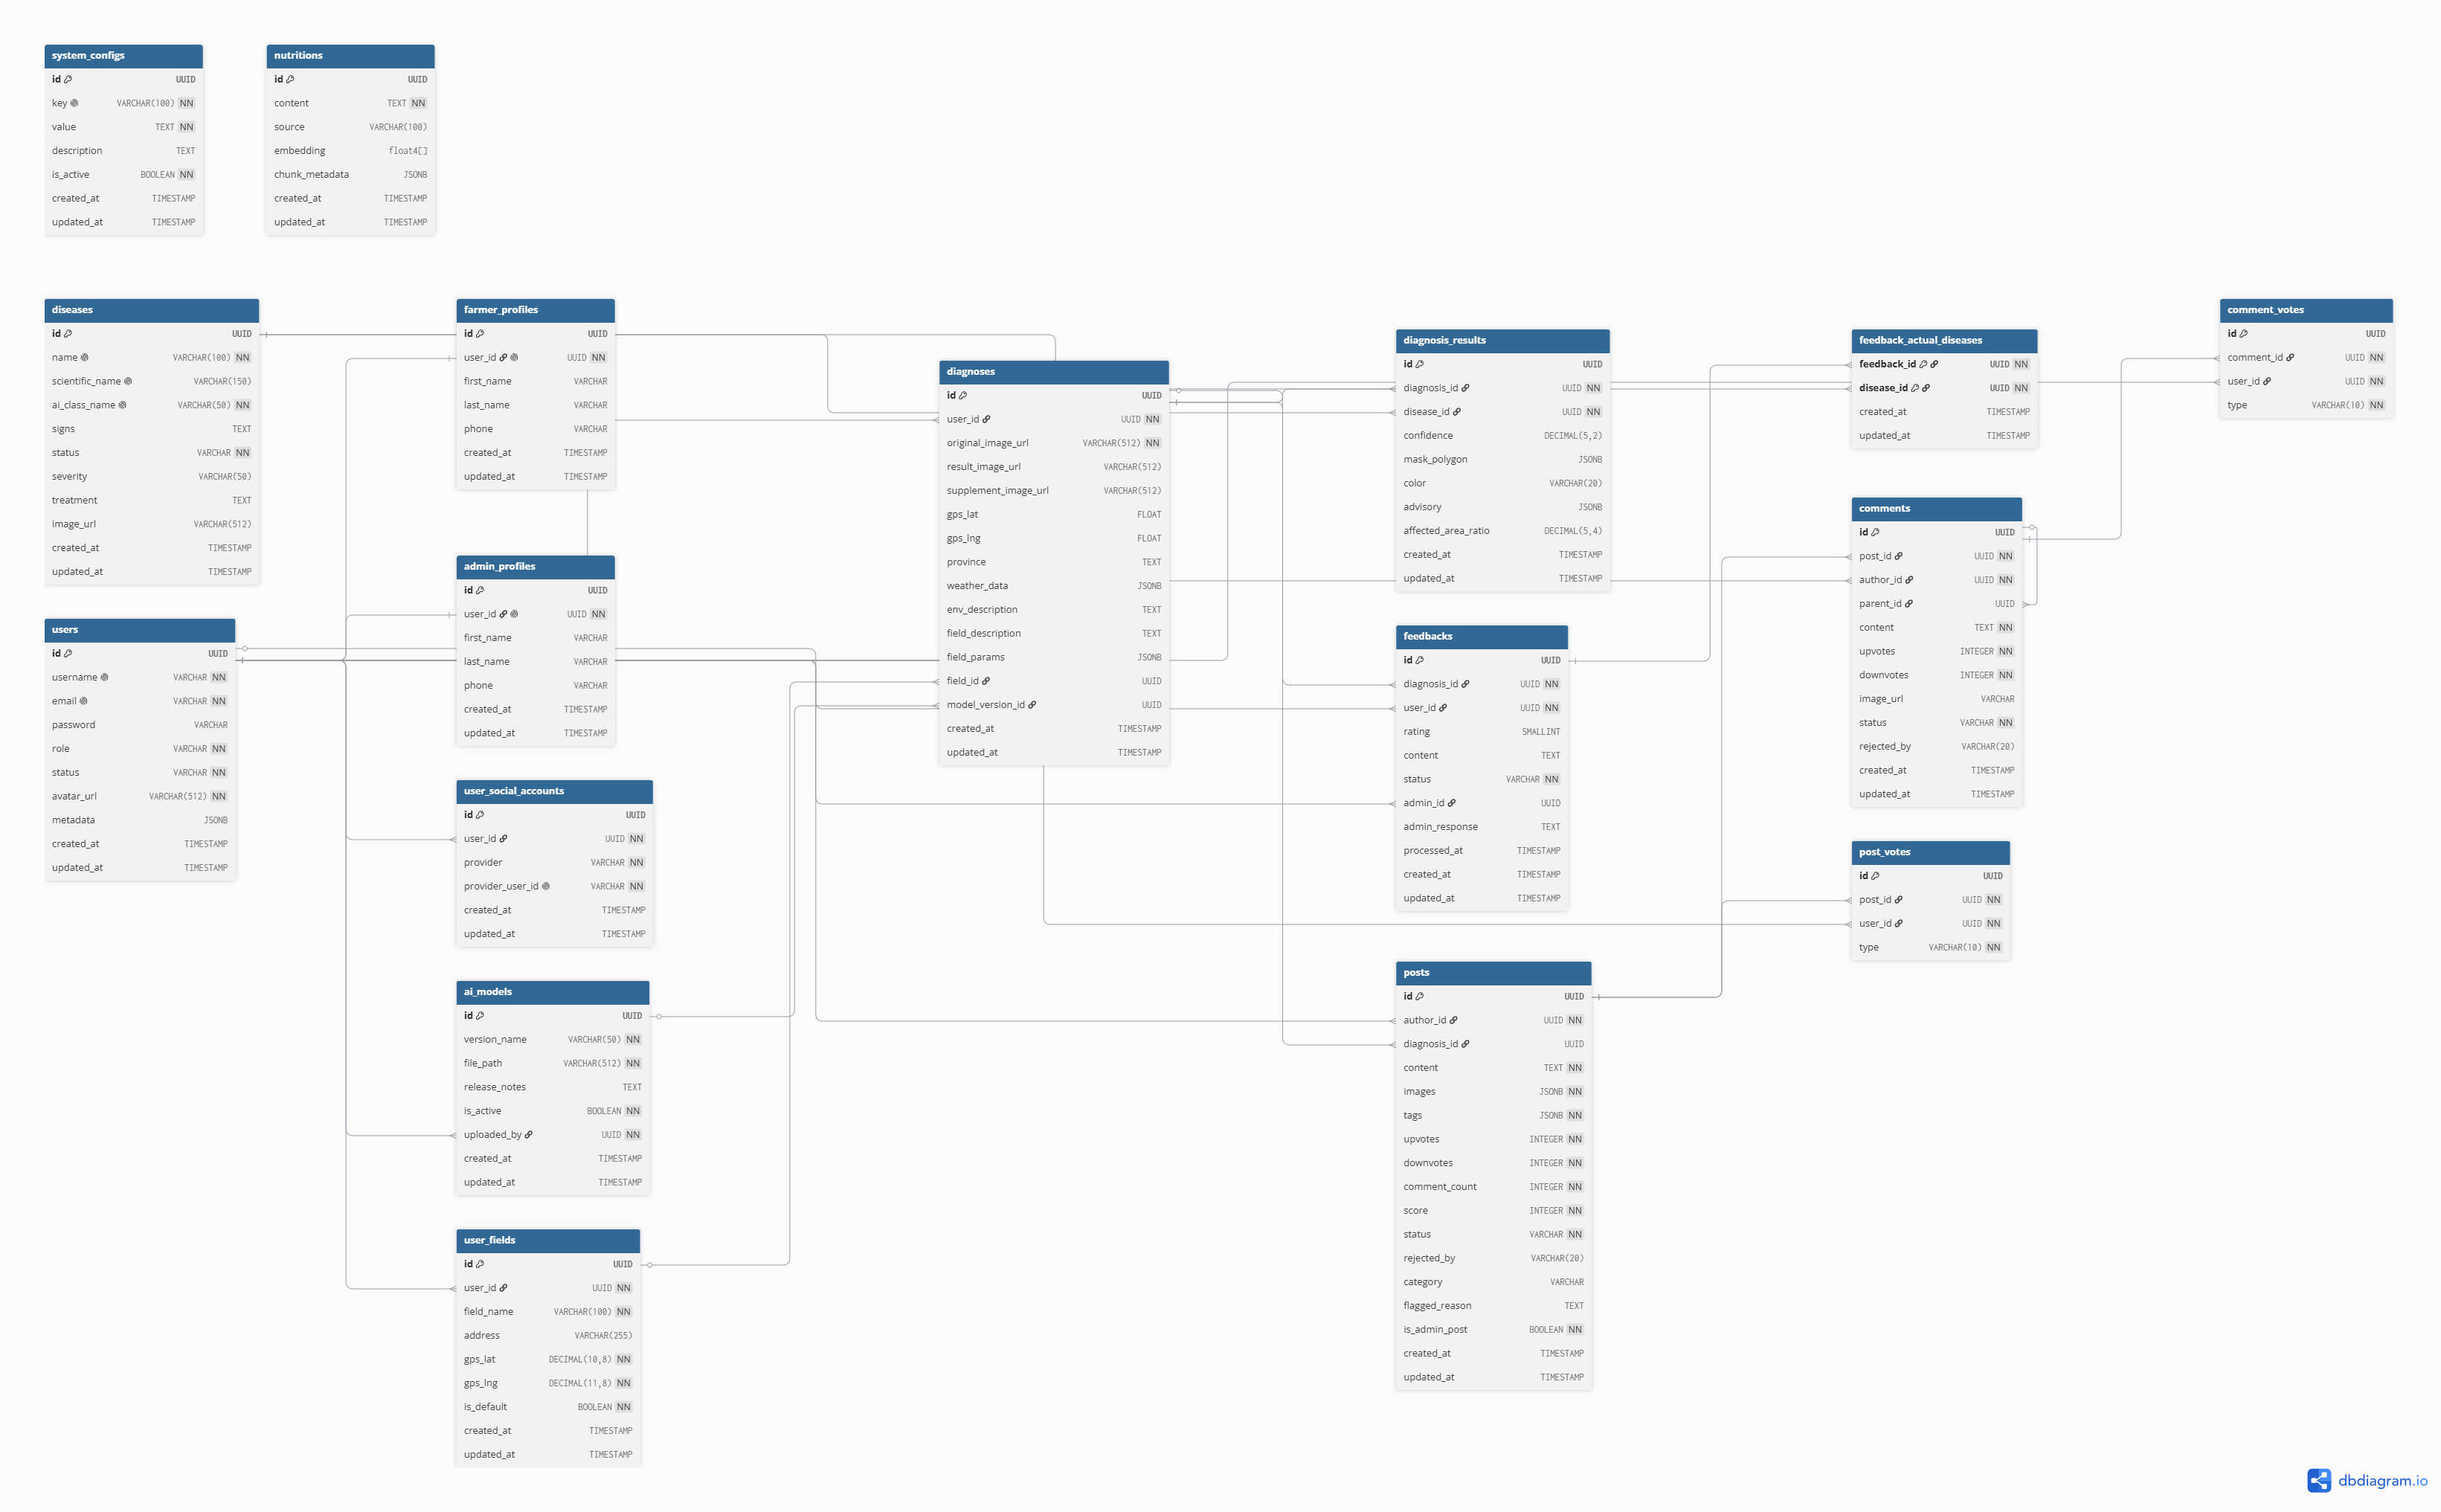
\includegraphics[width=\textwidth,height=0.85\textheight,keepaspectratio]{erd.png}
    \caption{Sơ đồ quan hệ thực thể (ERD)}
    \label{fig:erd}
\end{figure}

\hrulefill

% ============================================================
\section{Giải thích thuật ngữ}

\begin{longtable}{|l|p{11.5cm}|}
    \caption{Giải thích các thuật ngữ chuyên ngành}                                                           \\
    \hline
    \rowcolor{headerblue}
    \textbf{Thuật ngữ}    & \textbf{Giải thích}                                                               \\
    \hline
    CNN                   & Mạng nơ-ron tích chập --- thuật toán AI chuyên phân tích hình ảnh.                \\
    \hline
    Instance Segmentation & Kỹ thuật AI khoanh vùng chính xác từng đối tượng bệnh trên ảnh (pixel-level).     \\
    \hline
    pgvector              & Phần mở rộng của PostgreSQL cho phép tìm kiếm ngữ nghĩa trên dữ liệu văn bản.     \\
    \hline
    Embedding             & Biểu diễn số của văn bản để máy hiểu nghĩa, phục vụ tìm kiếm thông minh.          \\
    \hline
    RAG                   & Retrieval-Augmented Generation --- truy xuất tri thức để AI tư vấn chính xác hơn. \\
    \hline
    Redis                 & Bộ nhớ đệm tốc độ cao, dùng lưu tạm OTP và đếm lần đăng nhập sai.                 \\
    \hline
    JWT                   & Mã thông báo xác thực, giữ trạng thái đăng nhập của người dùng.                   \\
    \hline
    Bcrypt                & Thuật toán mã hóa mật khẩu một chiều, không thể giải ngược.                       \\
    \hline
    OTP                   & Mã xác thực dùng một lần, gửi qua email, hết hạn sau 10 phút.                     \\
    \hline
    GPS                   & Hệ thống định vị toàn cầu, xác định tọa độ vị trí người dùng.                     \\
    \hline
    Hot-swap              & Thay thế mô hình AI mà không cần tắt hệ thống.                                    \\
    \hline
    ERD                   & Sơ đồ thực thể quan hệ --- mô tả cấu trúc và quan hệ giữa các bảng dữ liệu.       \\
    \hline
    mask\_polygon         & Mảng tọa độ đa giác mô tả đường viền vùng bệnh trên ảnh.                          \\
    \hline
\end{longtable}

\end{document}
